\documentclass{article}%
\usepackage[T1]{fontenc}%
\usepackage[utf8]{inputenc}%
\usepackage{lmodern}%
\usepackage{textcomp}%
\usepackage{lastpage}%
\usepackage[tmargin=1in,lmargin=1in,textwidth=6.5in,textheight=9in]{geometry}%
\usepackage{graphicx}%
\usepackage{ragged2e}%
\usepackage{amsmath}%
%
\usepackage{times}%
\usepackage{hyperref}%
\hypersetup{colorlinks}%
\title{USC Ground Truth Documentation}%
\date{\today}%
%
\begin{document}%
\normalsize%
\maketitle%
\clearpage%
\tableofcontents%
\clearpage%
\section{Background}%
\label{sec:Background}%
We use influence diagrams as the underlying graph structure for our ground truth. Here is a simple influence diagram for a simulation of two actors, showing the three types of nodes and some possible links (always directed) among them:%


\begin{figure}[ht]%
\centering%
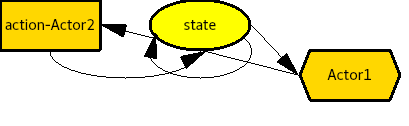
\includegraphics[width=0.8\textwidth]{/home/david/psychsim/tools/simple.png}%
\caption{Simple influence diagram}%
\end{figure}

%
\begin{itemize}%
\item%
Rectangular nodes are possible actions for a particular agent (``Actor 1'', indicated by color) representing a potential behavior. They are labeled with a verb (``action'') and an optional object of the verb (``Actor2''). An action node has a binary value, indicating whether or not the action was chosen.%
\item%
Oval nodes are state variables. Their value is potentially a probability distribution over a domain of possible values. All true state variables will be certain (i.e., 100\textbackslash{}\% probability for a single value), but agents' perceptions of the true state will often be uncertain.%
\item%
Hexagonal nodes are utility or reward nodes. They represent an expected value computation by the agent (``Actor1''). The node's value is a table with each row corresponding to a possible action choice and its expected utility.%
\item%
Links from action nodes to state nodes specify an effect that the action has on the value of the state.%
\item%
Links from one state node to another specify an influence that the value of the first state node has on the effect of at least one action on the second state node.%
\item%
Links from a state node to an agent's utility node specify that the state node is an input to the expected value calculation performed by that agent. There is a real{-}valued weight from \$(0,1\textbackslash{}{]}\$ on each link specifying the priority of that variable's influence on that agent's reward calculation (higher values mean higher priority).%
\item%
Links from utility nodes to action nodes indicate that the expected value calculation then determines whether or not that action is chosen. In the simulations described here, we use a strict maximization, so that the action choice is deterministic (i.e., the action with the highest expected value is performed, with ties broken by a pre{-}determined fixed order).%
\item%
Therefore, in the above simple ground truth, whether or not ``Actor1'' chooses to do ``action'' to ``Actor2'' influences the subsequent value of the variable ``state'' (link from rectangle to oval). The subsequent value of ``state'' also depends on its prior value (link from oval to itself). ``Actor1'''s expected value of doing ``action'' to ``Actor2'' is a function of the value of ``state'' (link from oval to hexagon), and this expected value influences whether or not ``Actor1'' chooses to do so (link from hexagon to rectangle).%
\end{itemize}%
Any real values (e.g., initial values of variables, conditional probability table values, reward weights) will be drawn from either a set \{0, 0.5, 1\} or \{0, 0.2, 0.4, 0.6, 0.8, 1\}, depending on the appropriate granularity needed.

%
\section{State}%
\label{sec:State}%
\subsection{Actor's age}%
\label{subsec:Actor's age}%
\begin{description}%
\item[Type:]%
Integer%
\end{description}

%
\subsection{Actor's alive}%
\label{subsec:Actor's alive}%
\begin{description}%
\item[Type:]%
Boolean%
\end{description}%


\begin{figure}[ht]%
\centering%
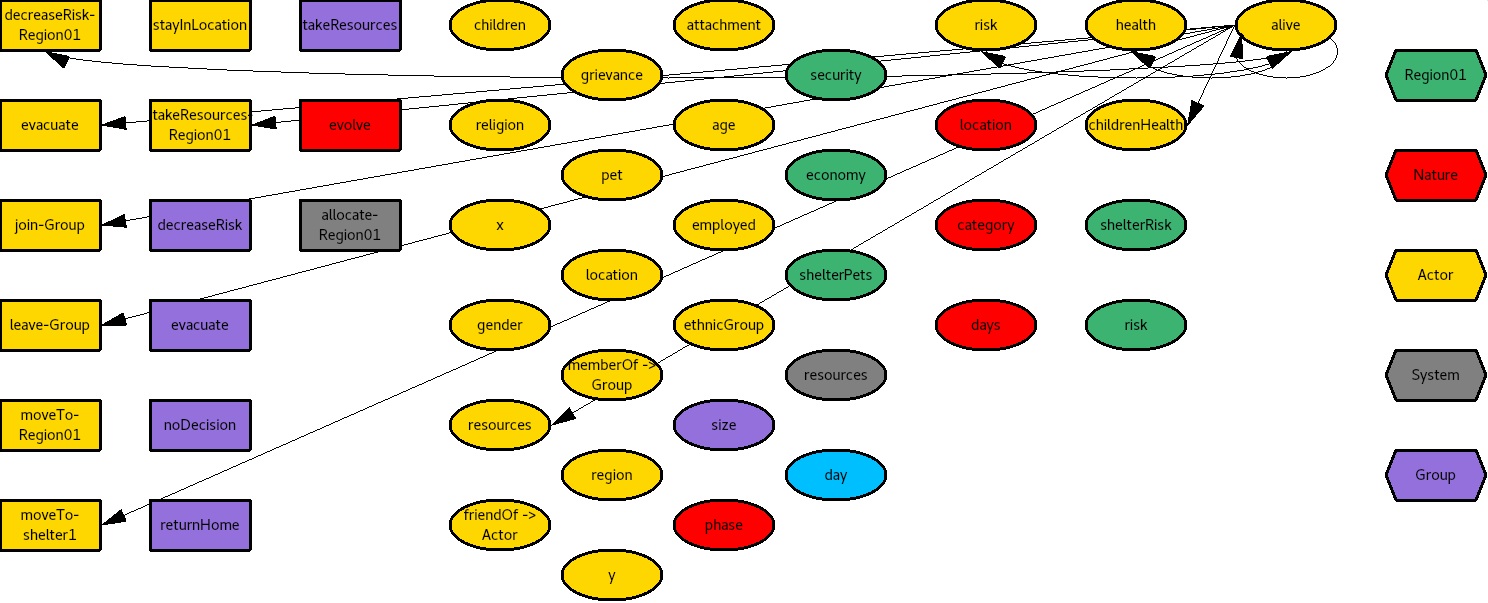
\includegraphics[width=0.8\textwidth]{images/aliveOfActor.png}%
\caption{Ground Truth subgraph for Actor's alive}%
\end{figure}

%
\subsubsection{Default change in Actor's alive}%
\label{ssubsec:Default change in Actor's alive}%
\begin{flushleft}%
IF %
\textbf{Actor's alive}%
\linebreak%
\hspace*{2em}%
THEN %
IF %
$\mbox{\textbf{Actor's health}} '$%
$>$%
0.01%
\linebreak%
\hspace*{4em}%
THEN %
$\mbox{\textbf{Actor's alive}} '$%
$\leftarrow$%
\textbf{true}%
\linebreak%
\hspace*{4em}%
ELSE %
$\mbox{\textbf{Actor's alive}} '$%
$\leftarrow$%
\textbf{false}%
\linebreak%
\hspace*{2em}%
ELSE %
$\mbox{\textbf{Actor's alive}} '$%
$\leftarrow$%
\textbf{Actor's alive}%
\end{flushleft}

%
\subsection{Actor's attachment}%
\label{subsec:Actor's attachment}%
Attachment style%
\begin{description}%
\item[Type:]%
String%
\item[Values:]%
\textbf{anxious}%
, %
\textbf{avoidant}%
, %
\textbf{secure}%
\end{description}%


\begin{figure}[ht]%
\centering%
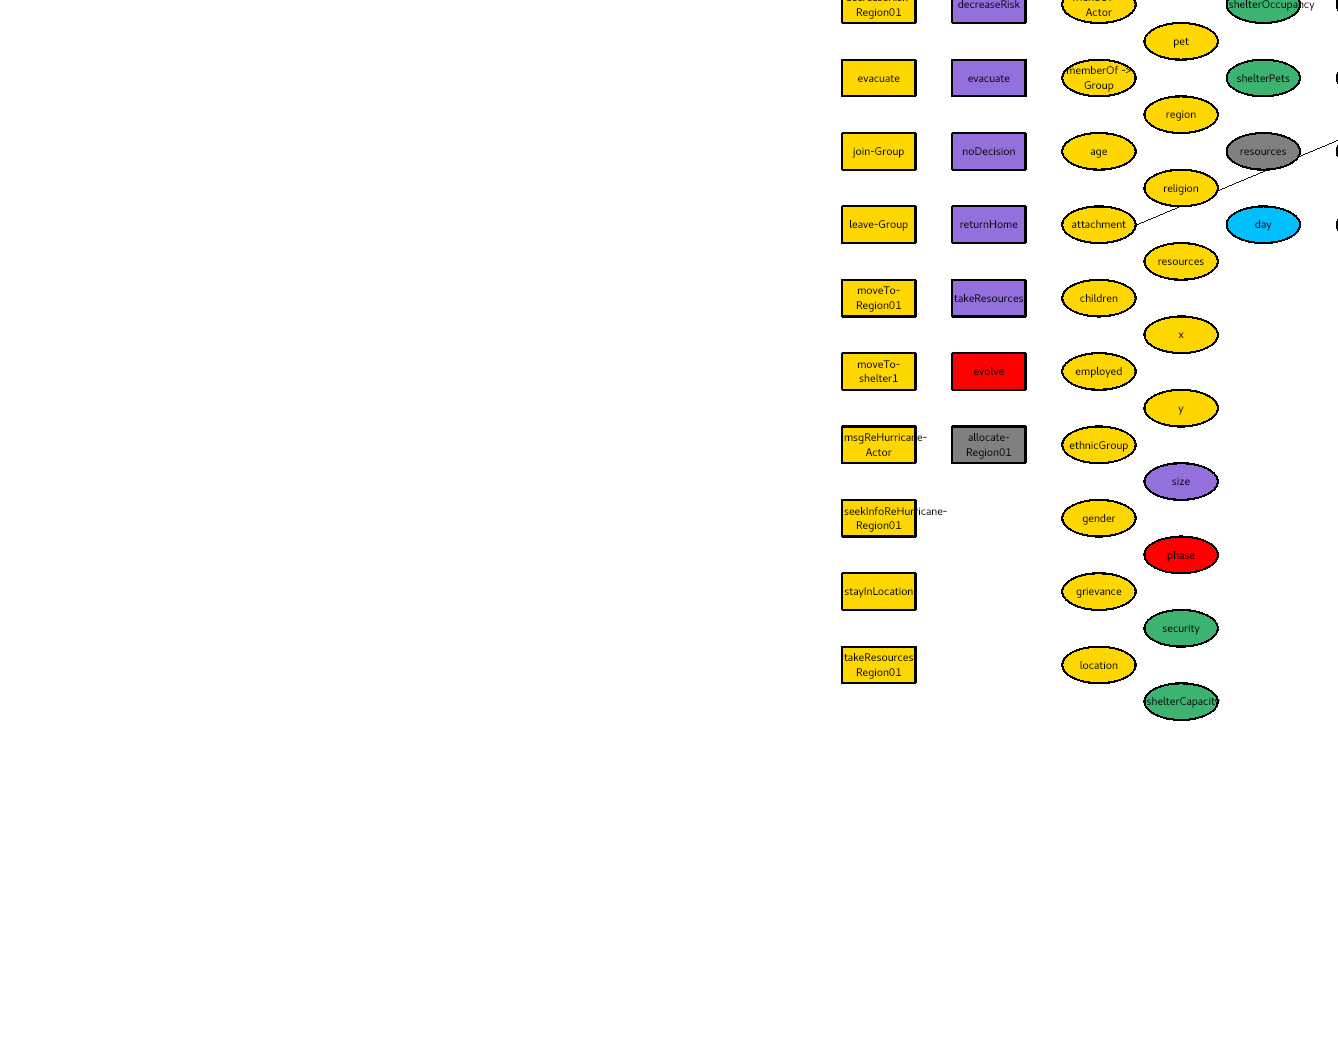
\includegraphics[width=0.8\textwidth]{images/attachmentOfActor.png}%
\caption{Ground Truth subgraph for Actor's attachment}%
\end{figure}

%
\subsection{Actor's category}%
\label{subsec:Actor's category}%
\begin{description}%
\item[Type:]%
Integer%
\end{description}

%
\subsection{Actor's center}%
\label{subsec:Actor's center}%
\begin{description}%
\item[Type:]%
String%
\item[Values:]%
\textbf{Region01}%
, %
\textbf{none}%
\end{description}

%
\subsection{Actor's children}%
\label{subsec:Actor's children}%
Number of children%
\begin{description}%
\item[Type:]%
Real%
\end{description}%


\begin{figure}[ht]%
\centering%
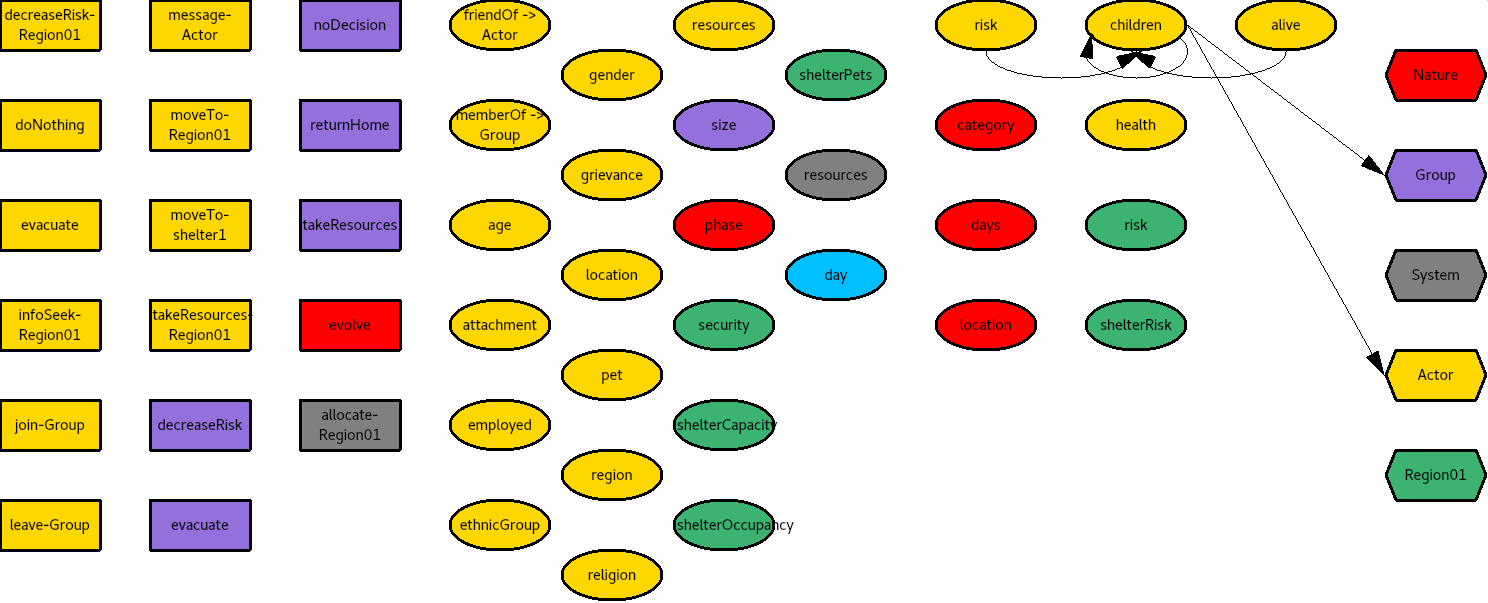
\includegraphics[width=0.8\textwidth]{images/childrenOfActor.png}%
\caption{Ground Truth subgraph for Actor's children}%
\end{figure}

%
\subsection{Actor's childrenHealth}%
\label{subsec:Actor's childrenHealth}%
Current level of children's physical wellbeing%
\begin{description}%
\item[Type:]%
Real%
\end{description}%


\begin{figure}[ht]%
\centering%
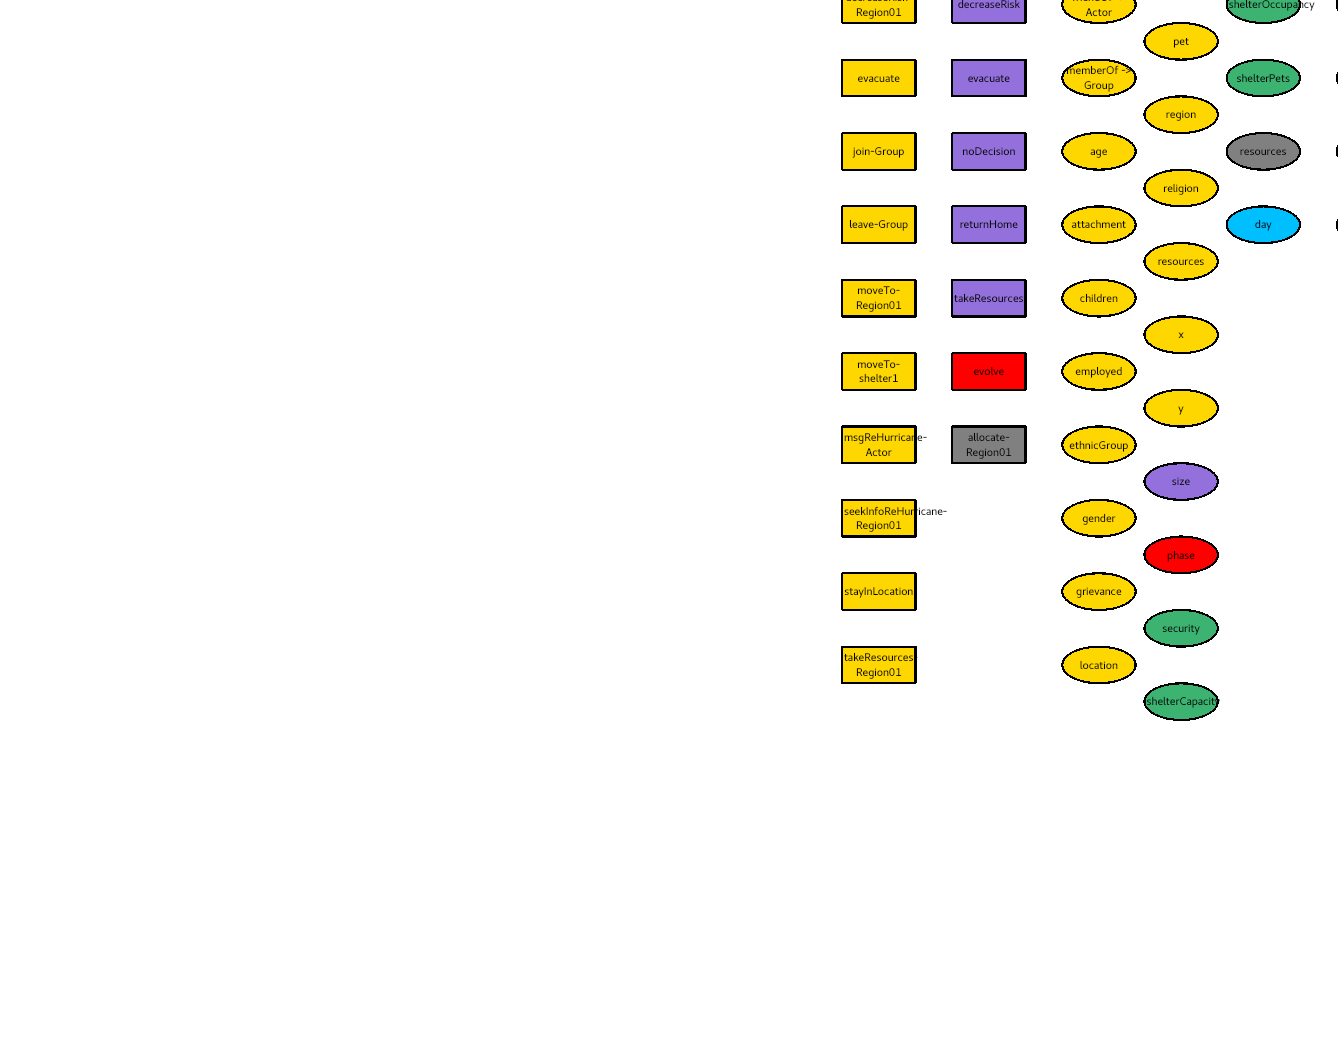
\includegraphics[width=0.8\textwidth]{images/childrenHealthOfActor.png}%
\caption{Ground Truth subgraph for Actor's childrenHealth}%
\end{figure}

%
\subsubsection{Default change in Actor's childrenHealth}%
\label{ssubsec:Default change in Actor's childrenHealth}%
\begin{flushleft}%
IF %
\textbf{Actor's alive}%
\linebreak%
\hspace*{2em}%
THEN %
IF %
$\mbox{\textbf{Actor's risk}} '$%
$>$%
{[}0.2,0.4,0.6,0.8,1.0{]}%
\linebreak%
\hspace*{4em}%
$\mbox{\textbf{Actor's childrenHealth}} '$%
$\leftarrow$%
60\%%
$\cdot$%
\textbf{Actor's childrenHealth}%
+0.24%
\linebreak%
\hspace*{4em}%
1 %
\linebreak%
\hspace*{6em}%
20\%: %
$\mbox{\textbf{Actor's childrenHealth}} '$%
$\leftarrow$%
60\%%
$\cdot$%
\textbf{Actor's childrenHealth}%
\linebreak%
\hspace*{6em}%
80\%: %
$\mbox{\textbf{Actor's childrenHealth}} '$%
$\leftarrow$%
60\%%
$\cdot$%
\textbf{Actor's childrenHealth}%
+0.24%
\linebreak%
\hspace*{4em}%
2 %
\linebreak%
\hspace*{6em}%
40\%: %
$\mbox{\textbf{Actor's childrenHealth}} '$%
$\leftarrow$%
60\%%
$\cdot$%
\textbf{Actor's childrenHealth}%
\linebreak%
\hspace*{6em}%
60\%: %
$\mbox{\textbf{Actor's childrenHealth}} '$%
$\leftarrow$%
60\%%
$\cdot$%
\textbf{Actor's childrenHealth}%
+0.24%
\linebreak%
\hspace*{4em}%
3 %
\linebreak%
\hspace*{6em}%
60\%: %
$\mbox{\textbf{Actor's childrenHealth}} '$%
$\leftarrow$%
60\%%
$\cdot$%
\textbf{Actor's childrenHealth}%
\linebreak%
\hspace*{6em}%
40\%: %
$\mbox{\textbf{Actor's childrenHealth}} '$%
$\leftarrow$%
60\%%
$\cdot$%
\textbf{Actor's childrenHealth}%
+0.24%
\linebreak%
\hspace*{4em}%
4 %
\linebreak%
\hspace*{6em}%
80\%: %
$\mbox{\textbf{Actor's childrenHealth}} '$%
$\leftarrow$%
60\%%
$\cdot$%
\textbf{Actor's childrenHealth}%
\linebreak%
\hspace*{6em}%
19\%: %
$\mbox{\textbf{Actor's childrenHealth}} '$%
$\leftarrow$%
60\%%
$\cdot$%
\textbf{Actor's childrenHealth}%
+0.24%
\linebreak%
\hspace*{4em}%
5 %
\linebreak%
\hspace*{6em}%
100\%: %
$\mbox{\textbf{Actor's childrenHealth}} '$%
$\leftarrow$%
60\%%
$\cdot$%
\textbf{Actor's childrenHealth}%
\linebreak%
\hspace*{6em}%
0\%: %
$\mbox{\textbf{Actor's childrenHealth}} '$%
$\leftarrow$%
60\%%
$\cdot$%
\textbf{Actor's childrenHealth}%
+0.24%
\linebreak%
\hspace*{2em}%
ELSE %
$\mbox{\textbf{Actor's childrenHealth}} '$%
$\leftarrow$%
0.00%
\end{flushleft}

%
\subsection{Actor's days}%
\label{subsec:Actor's days}%
\begin{description}%
\item[Type:]%
Integer%
\end{description}

%
\subsection{Actor's employed}%
\label{subsec:Actor's employed}%
Has a full{-}time job%
\begin{description}%
\item[Type:]%
Boolean%
\end{description}%


\begin{figure}[ht]%
\centering%
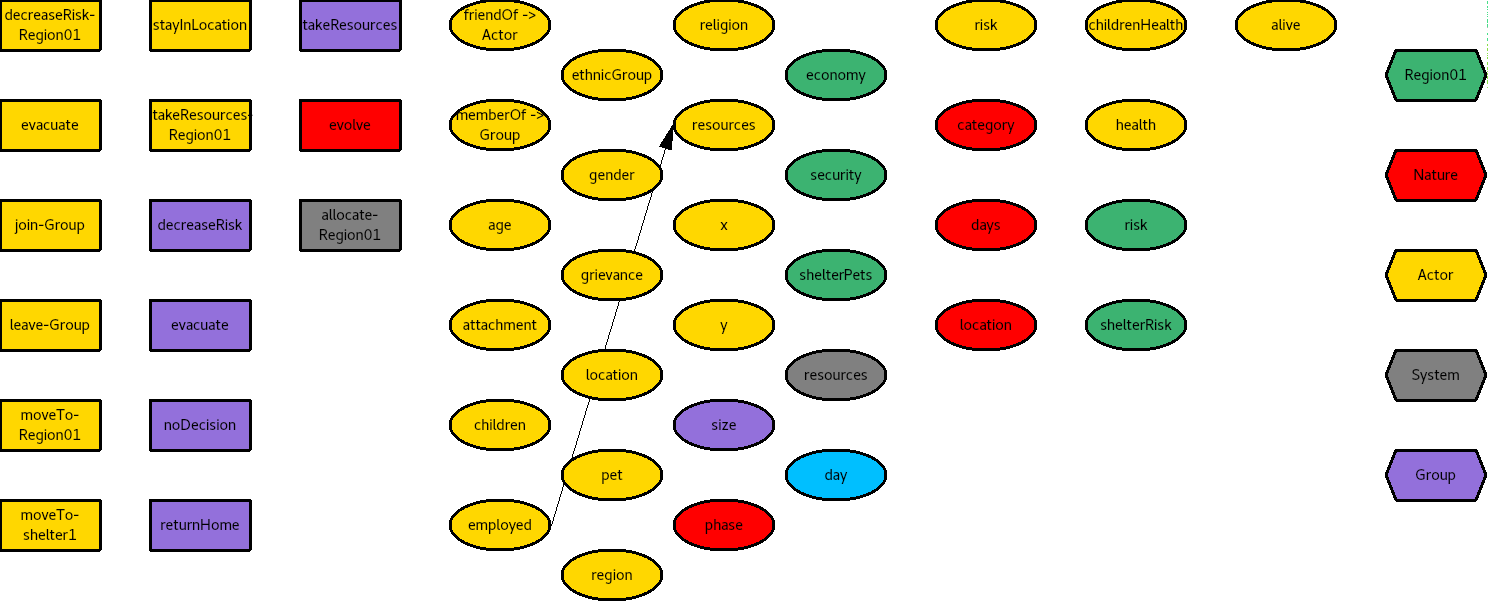
\includegraphics[width=0.8\textwidth]{images/employedOfActor.png}%
\caption{Ground Truth subgraph for Actor's employed}%
\end{figure}

%
\subsection{Actor's ethnicGroup}%
\label{subsec:Actor's ethnicGroup}%
Ethnicity of actor%
\begin{description}%
\item[Type:]%
String%
\item[Values:]%
\textbf{majority}%
, %
\textbf{minority}%
\end{description}

%
\subsection{Actor's gender}%
\label{subsec:Actor's gender}%
\begin{description}%
\item[Type:]%
String%
\item[Values:]%
\textbf{female}%
, %
\textbf{male}%
\end{description}

%
\subsection{Actor's grievance}%
\label{subsec:Actor's grievance}%
Current level of grievance felt toward system%
\begin{description}%
\item[Type:]%
Real%
\end{description}%


\begin{figure}[ht]%
\centering%
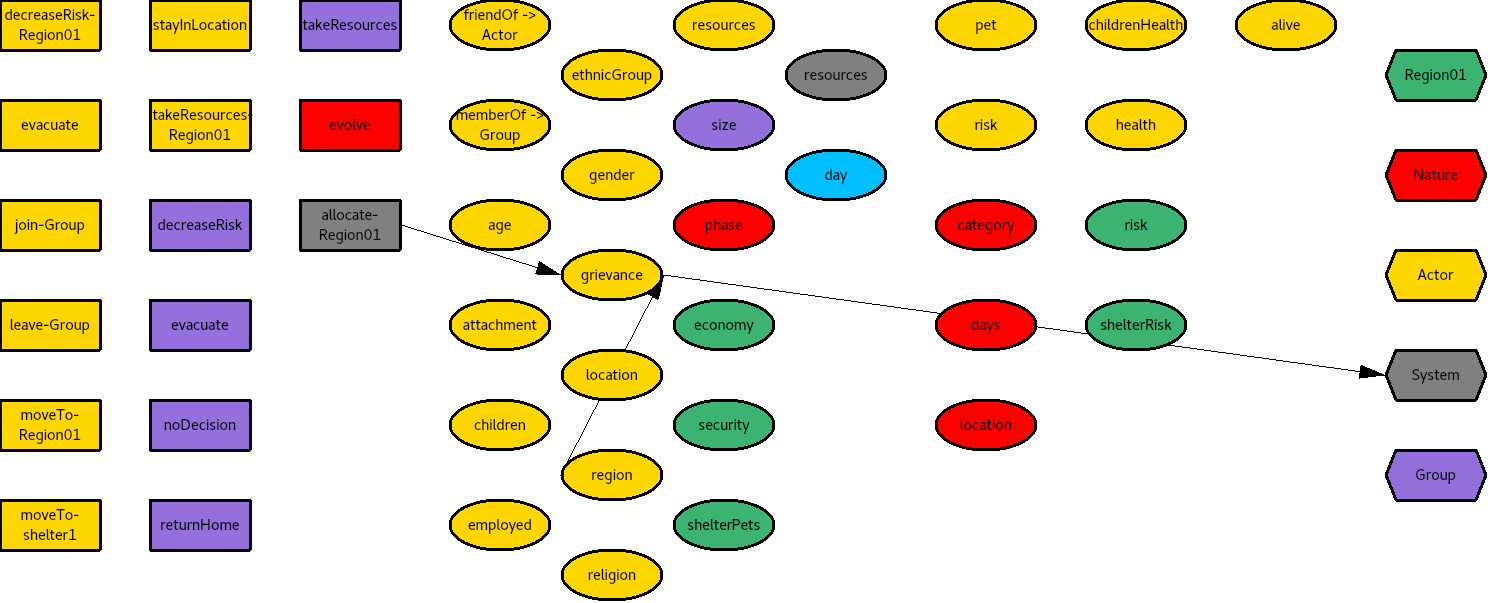
\includegraphics[width=0.8\textwidth]{images/grievanceOfActor.png}%
\caption{Ground Truth subgraph for Actor's grievance}%
\end{figure}

%
\subsection{Actor's health}%
\label{subsec:Actor's health}%
Current level of physical wellbeing%
\begin{description}%
\item[Type:]%
Real%
\end{description}%


\begin{figure}[ht]%
\centering%
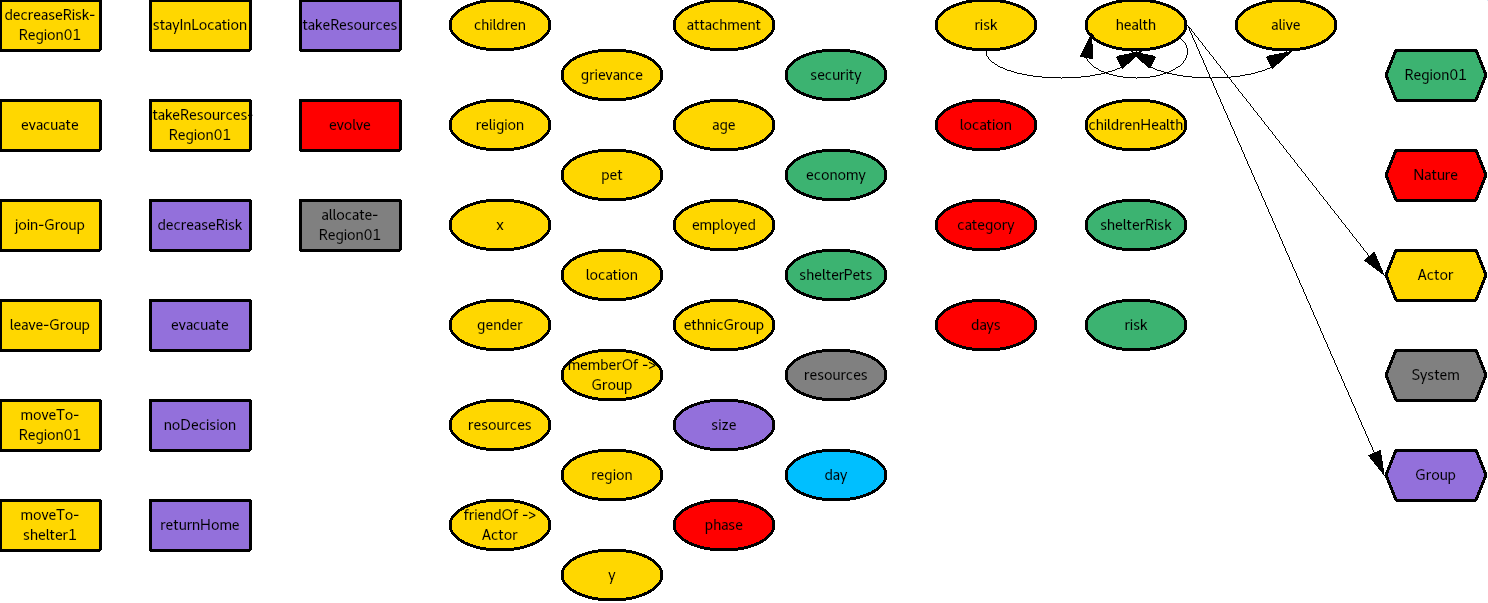
\includegraphics[width=0.8\textwidth]{images/healthOfActor.png}%
\caption{Ground Truth subgraph for Actor's health}%
\end{figure}

%
\subsubsection{Default change in Actor's health}%
\label{ssubsec:Default change in Actor's health}%
\begin{flushleft}%
IF %
\textbf{Actor's alive}%
\linebreak%
\hspace*{2em}%
THEN %
IF %
$\mbox{\textbf{Actor's risk}} '$%
$>$%
{[}0.2,0.4,0.6,0.8,1.0{]}%
\linebreak%
\hspace*{4em}%
$\mbox{\textbf{Actor's health}} '$%
$\leftarrow$%
60\%%
$\cdot$%
\textbf{Actor's health}%
+0.24%
\linebreak%
\hspace*{4em}%
1 %
\linebreak%
\hspace*{6em}%
20\%: %
$\mbox{\textbf{Actor's health}} '$%
$\leftarrow$%
60\%%
$\cdot$%
\textbf{Actor's health}%
\linebreak%
\hspace*{6em}%
80\%: %
$\mbox{\textbf{Actor's health}} '$%
$\leftarrow$%
60\%%
$\cdot$%
\textbf{Actor's health}%
+0.24%
\linebreak%
\hspace*{4em}%
2 %
\linebreak%
\hspace*{6em}%
40\%: %
$\mbox{\textbf{Actor's health}} '$%
$\leftarrow$%
60\%%
$\cdot$%
\textbf{Actor's health}%
\linebreak%
\hspace*{6em}%
60\%: %
$\mbox{\textbf{Actor's health}} '$%
$\leftarrow$%
60\%%
$\cdot$%
\textbf{Actor's health}%
+0.24%
\linebreak%
\hspace*{4em}%
3 %
\linebreak%
\hspace*{6em}%
60\%: %
$\mbox{\textbf{Actor's health}} '$%
$\leftarrow$%
60\%%
$\cdot$%
\textbf{Actor's health}%
\linebreak%
\hspace*{6em}%
40\%: %
$\mbox{\textbf{Actor's health}} '$%
$\leftarrow$%
60\%%
$\cdot$%
\textbf{Actor's health}%
+0.24%
\linebreak%
\hspace*{4em}%
4 %
\linebreak%
\hspace*{6em}%
80\%: %
$\mbox{\textbf{Actor's health}} '$%
$\leftarrow$%
60\%%
$\cdot$%
\textbf{Actor's health}%
\linebreak%
\hspace*{6em}%
19\%: %
$\mbox{\textbf{Actor's health}} '$%
$\leftarrow$%
60\%%
$\cdot$%
\textbf{Actor's health}%
+0.24%
\linebreak%
\hspace*{4em}%
5 %
\linebreak%
\hspace*{6em}%
100\%: %
$\mbox{\textbf{Actor's health}} '$%
$\leftarrow$%
60\%%
$\cdot$%
\textbf{Actor's health}%
\linebreak%
\hspace*{6em}%
0\%: %
$\mbox{\textbf{Actor's health}} '$%
$\leftarrow$%
60\%%
$\cdot$%
\textbf{Actor's health}%
+0.24%
\linebreak%
\hspace*{2em}%
ELSE %
$\mbox{\textbf{Actor's health}} '$%
$\leftarrow$%
0.00%
\end{flushleft}

%
\subsection{Actor's location}%
\label{subsec:Actor's location}%
Current location%
\begin{description}%
\item[Type:]%
String%
\item[Values:]%
\textbf{Region01}%
, %
\textbf{evacuated}%
, %
\textbf{shelter1}%
\end{description}%


\begin{figure}[ht]%
\centering%
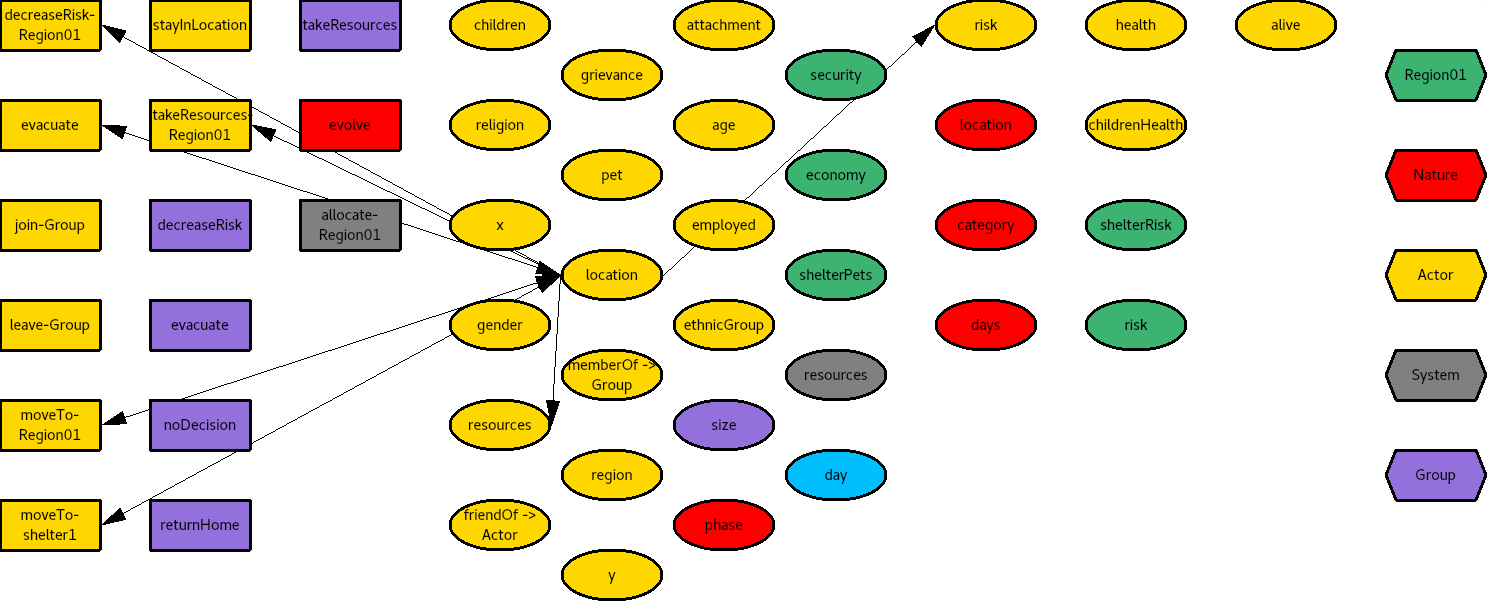
\includegraphics[width=0.8\textwidth]{images/locationOfActor.png}%
\caption{Ground Truth subgraph for Actor's location}%
\end{figure}

%
\subsubsection{Effect of Actor{-}evacuate on Actor's location}%
\label{ssubsec:Effect of Actor{-}evacuate on Actor's location}%
\begin{flushleft}%
$\mbox{\textbf{Actor's location}} '$%
$\leftarrow$%
\textbf{evacuated}%
\end{flushleft}

%
\subsubsection{Effect of Actor{-}moveTo{-}Region01 on Actor's location}%
\label{ssubsec:Effect of Actor{-}moveTo{-}Region01 on Actor's location}%
\begin{flushleft}%
$\mbox{\textbf{Actor's location}} '$%
$\leftarrow$%
\textbf{Region01}%
\end{flushleft}

%
\subsubsection{Effect of Actor{-}moveTo{-}shelter1 on Actor's location}%
\label{ssubsec:Effect of Actor{-}moveTo{-}shelter1 on Actor's location}%
\begin{flushleft}%
$\mbox{\textbf{Actor's location}} '$%
$\leftarrow$%
\textbf{shelter1}%
\end{flushleft}

%
\subsection{Actor's perceivedChildrenHealth}%
\label{subsec:Actor's perceivedChildrenHealth}%
\begin{description}%
\item[Type:]%
Real%
\end{description}

%
\subsection{Actor's perceivedHealth}%
\label{subsec:Actor's perceivedHealth}%
\begin{description}%
\item[Type:]%
Real%
\end{description}

%
\subsection{Actor's pet}%
\label{subsec:Actor's pet}%
Owns a pet%
\begin{description}%
\item[Type:]%
Boolean%
\end{description}

%
\subsection{Actor's phase}%
\label{subsec:Actor's phase}%
\begin{description}%
\item[Type:]%
String%
\item[Values:]%
\textbf{active}%
, %
\textbf{approaching}%
, %
\textbf{none}%
\end{description}

%
\subsection{Actor's region}%
\label{subsec:Actor's region}%
Region of residence%
\begin{description}%
\item[Type:]%
String%
\item[Values:]%
\textbf{Region01}%
\end{description}%


\begin{figure}[ht]%
\centering%
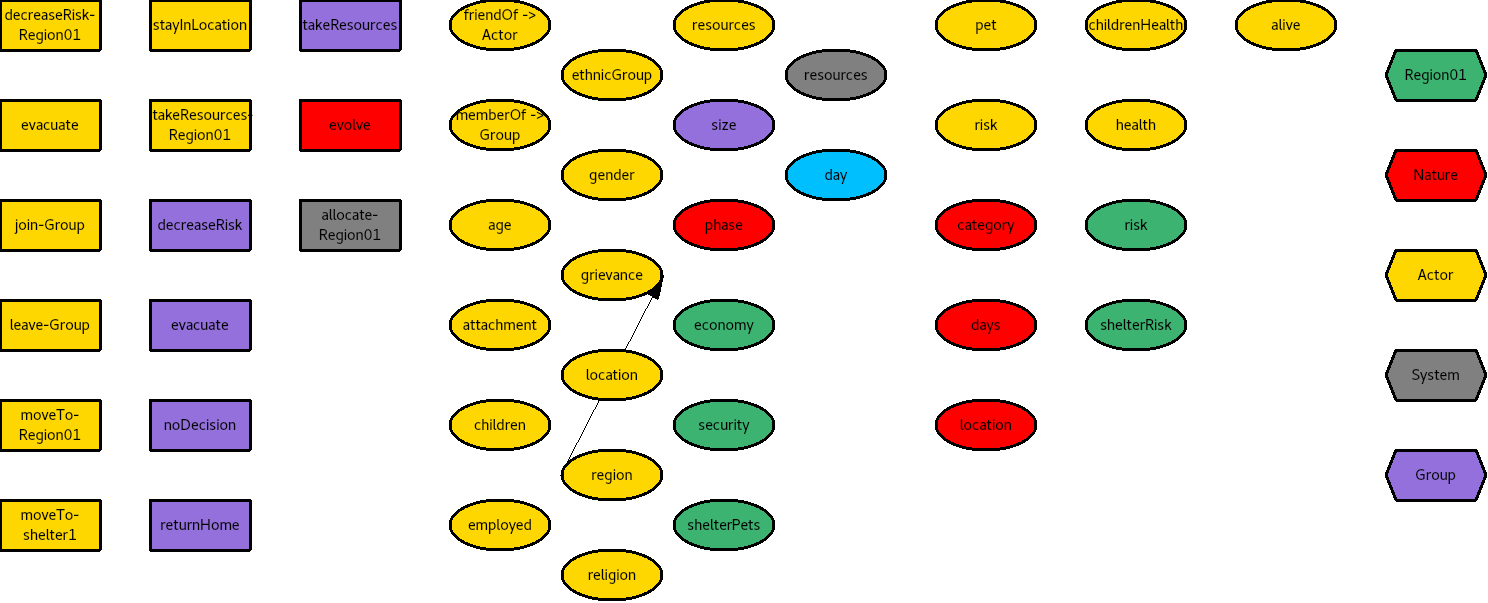
\includegraphics[width=0.8\textwidth]{images/regionOfActor.png}%
\caption{Ground Truth subgraph for Actor's region}%
\end{figure}

%
\subsection{Actor's religion}%
\label{subsec:Actor's religion}%
Religious affiliation of actor%
\begin{description}%
\item[Type:]%
String%
\item[Values:]%
\textbf{majority}%
, %
\textbf{minority}%
, %
\textbf{none}%
\end{description}

%
\subsection{Actor's resources}%
\label{subsec:Actor's resources}%
Material resources (wealth) currently owned%
\begin{description}%
\item[Type:]%
Real%
\end{description}%


\begin{figure}[ht]%
\centering%
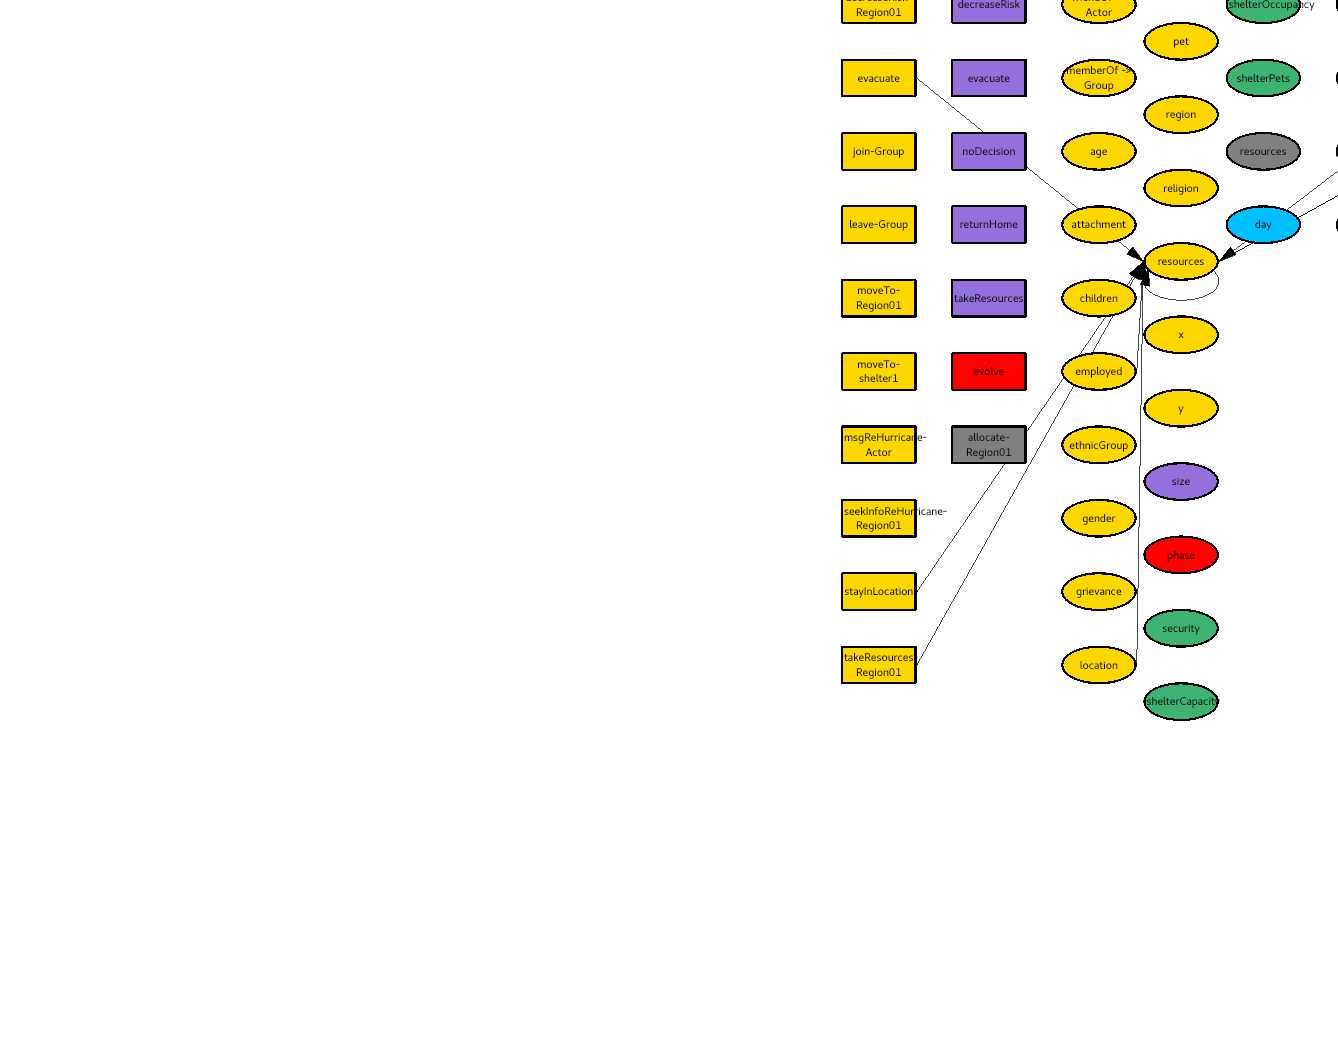
\includegraphics[width=0.8\textwidth]{images/resourcesOfActor.png}%
\caption{Ground Truth subgraph for Actor's resources}%
\end{figure}

%
\subsubsection{Effect of Actor{-}evacuate on Actor's resources}%
\label{ssubsec:Effect of Actor{-}evacuate on Actor's resources}%
\begin{flushleft}%
IF %
\textbf{Actor's resources}%
$>$%
0.20%
\linebreak%
\hspace*{2em}%
THEN %
$\mbox{\textbf{Actor's resources}} '$%
$\leftarrow$%
\textbf{Actor's resources}%
${-}0.20$%
\linebreak%
\hspace*{2em}%
ELSE %
$\mbox{\textbf{Actor's resources}} '$%
$\leftarrow$%
0.00%
\end{flushleft}

%
\subsubsection{Effect of Actor{-}moveTo{-}Region01 on Actor's resources}%
\label{ssubsec:Effect of Actor{-}moveTo{-}Region01 on Actor's resources}%
\begin{flushleft}%
IF %
\textbf{Actor's alive}%
\linebreak%
\hspace*{2em}%
THEN %
IF %
\textbf{Actor's employed}%
\linebreak%
\hspace*{4em}%
THEN %
$\mbox{\textbf{Actor's resources}} '$%
$\leftarrow$%
80\%%
$\cdot$%
\textbf{Actor's resources}%
+0.20%
\linebreak%
\hspace*{4em}%
ELSE %
$\mbox{\textbf{Actor's resources}} '$%
$\leftarrow$%
\textbf{Actor's resources}%
\linebreak%
\hspace*{2em}%
ELSE %
$\mbox{\textbf{Actor's resources}} '$%
$\leftarrow$%
\textbf{Actor's resources}%
\end{flushleft}

%
\subsubsection{Effect of Actor{-}stayInLocation on Actor's resources}%
\label{ssubsec:Effect of Actor{-}stayInLocation on Actor's resources}%
\begin{flushleft}%
IF %
\textbf{Actor's alive}%
\linebreak%
\hspace*{2em}%
THEN %
IF %
\textbf{Actor's employed}%
\linebreak%
\hspace*{4em}%
THEN %
IF %
\textbf{Actor's location}%
$=$%
\textbf{\{'Region01', 'evacuated'\}}%
\linebreak%
\hspace*{6em}%
THEN %
$\mbox{\textbf{Actor's resources}} '$%
$\leftarrow$%
80\%%
$\cdot$%
\textbf{Actor's resources}%
+0.20%
\linebreak%
\hspace*{6em}%
ELSE %
$\mbox{\textbf{Actor's resources}} '$%
$\leftarrow$%
\textbf{Actor's resources}%
\linebreak%
\hspace*{4em}%
ELSE %
$\mbox{\textbf{Actor's resources}} '$%
$\leftarrow$%
\textbf{Actor's resources}%
\linebreak%
\hspace*{2em}%
ELSE %
$\mbox{\textbf{Actor's resources}} '$%
$\leftarrow$%
\textbf{Actor's resources}%
\end{flushleft}

%
\subsubsection{Effect of Actor{-}takeResources{-}Region01 on Actor's resources}%
\label{ssubsec:Effect of Actor{-}takeResources{-}Region01 on Actor's resources}%
\begin{flushleft}%
$\mbox{\textbf{Actor's resources}} '$%
$\leftarrow$%
80\%%
$\cdot$%
\textbf{Actor's resources}%
+0.20%
\end{flushleft}

%
\subsection{Actor's risk}%
\label{subsec:Actor's risk}%
Current level of risk from hurricane%
\begin{description}%
\item[Type:]%
Real%
\end{description}%


\begin{figure}[ht]%
\centering%
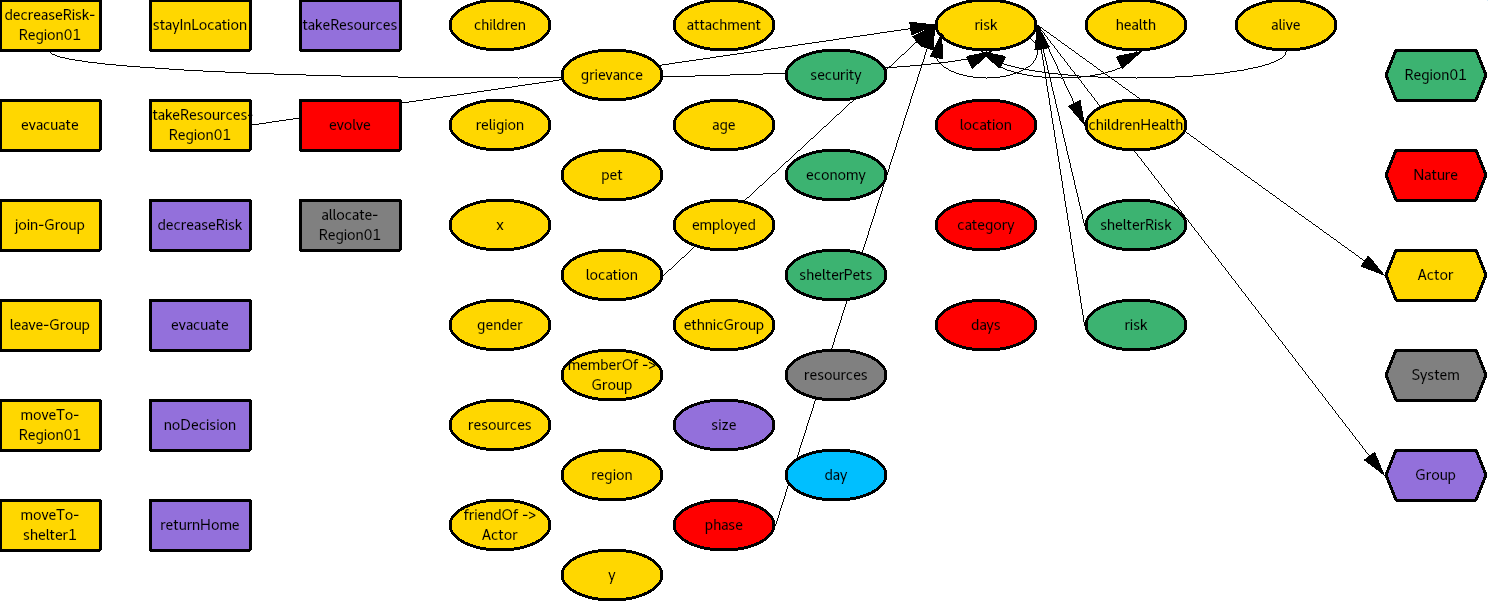
\includegraphics[width=0.8\textwidth]{images/riskOfActor.png}%
\caption{Ground Truth subgraph for Actor's risk}%
\end{figure}

%
\subsubsection{Effect of Actor{-}decreaseRisk{-}Region01 on Actor's risk}%
\label{ssubsec:Effect of Actor{-}decreaseRisk{-}Region01 on Actor's risk}%
\begin{flushleft}%
$\mbox{\textbf{Actor's risk}} '$%
$\leftarrow$%
80\%%
$\cdot$%
\textbf{Actor's risk}%
+0.20%
\end{flushleft}

%
\subsubsection{Effect of Actor{-}takeResources{-}Region01 on Actor's risk}%
\label{ssubsec:Effect of Actor{-}takeResources{-}Region01 on Actor's risk}%
\begin{flushleft}%
IF %
\textbf{Nature's phase}%
$=$%
\textbf{none}%
\linebreak%
\hspace*{2em}%
THEN %
$\mbox{\textbf{Actor's risk}} '$%
$\leftarrow$%
19\%%
$\cdot$%
\textbf{Actor's risk}%
+0.80%
\linebreak%
\hspace*{2em}%
ELSE %
$\mbox{\textbf{Actor's risk}} '$%
$\leftarrow$%
40\%%
$\cdot$%
\textbf{Actor's risk}%
+0.60%
\end{flushleft}

%
\subsubsection{Default change in Actor's risk}%
\label{ssubsec:Default change in Actor's risk}%
\begin{flushleft}%
IF %
\textbf{Actor's alive}%
\linebreak%
\hspace*{2em}%
THEN %
IF %
$\mbox{\textbf{Actor's location}} '$%
$=$%
\textbf{shelter1}%
\linebreak%
\hspace*{4em}%
THEN %
$\mbox{\textbf{Actor's risk}} '$%
$\leftarrow$%
\textbf{Region01's shelterRisk}%
\linebreak%
\hspace*{4em}%
ELSE %
IF %
$\mbox{\textbf{Actor's location}} '$%
$=$%
\textbf{evacuated}%
\linebreak%
\hspace*{6em}%
THEN %
$\mbox{\textbf{Actor's risk}} '$%
$\leftarrow$%
9\%%
$\cdot$%
\textbf{Actor's risk}%
\linebreak%
\hspace*{6em}%
ELSE %
$\mbox{\textbf{Actor's risk}} '$%
$\leftarrow$%
\textbf{Region01's risk}%
\linebreak%
\hspace*{2em}%
ELSE %
$\mbox{\textbf{Actor's risk}} '$%
$\leftarrow$%
0.00%
\end{flushleft}

%
\subsection{Actor's x}%
\label{subsec:Actor's x}%
Representation of residence's longitude%
\begin{description}%
\item[Type:]%
Real%
\end{description}

%
\subsection{Actor's y}%
\label{subsec:Actor's y}%
Representation of residence's latitude%
\begin{description}%
\item[Type:]%
Real%
\end{description}

%
\subsection{Group's size}%
\label{subsec:Group's size}%
\begin{description}%
\item[Type:]%
Integer%
\end{description}%


\begin{figure}[ht]%
\centering%
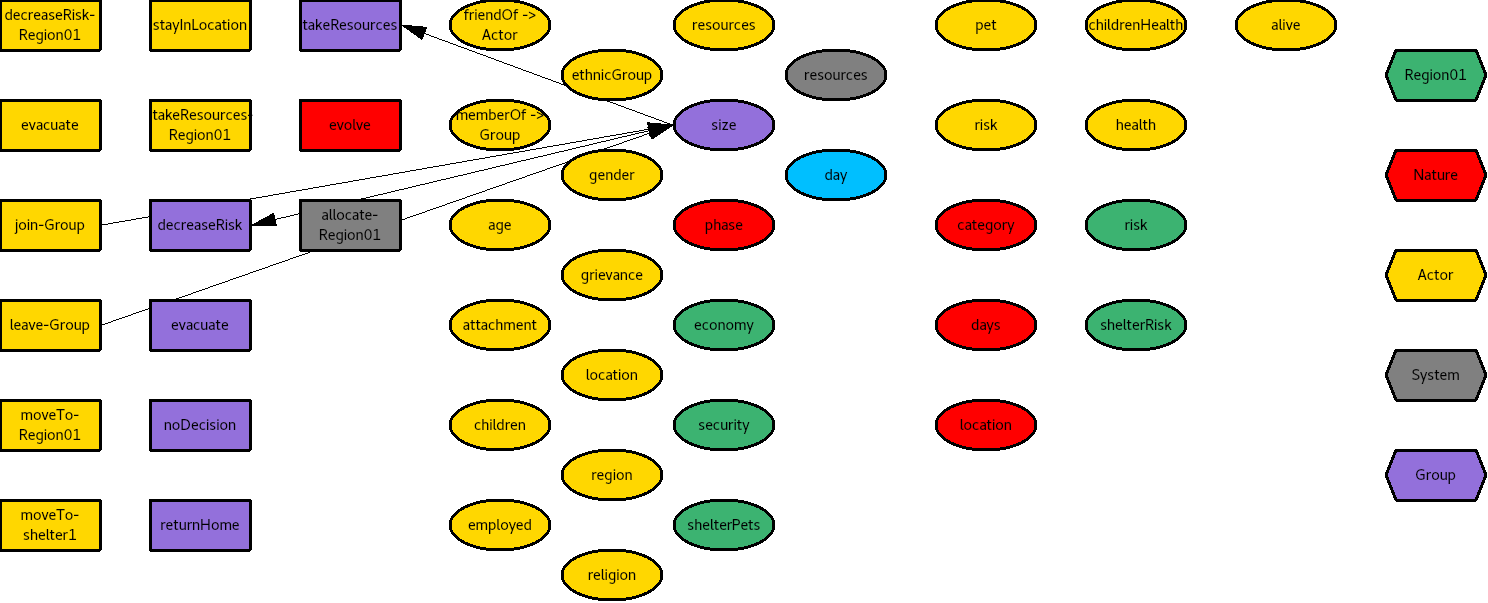
\includegraphics[width=0.8\textwidth]{images/sizeOfGroup.png}%
\caption{Ground Truth subgraph for Group's size}%
\end{figure}

%
\subsubsection{Effect of Actor{-}join{-}Group on Group's size}%
\label{ssubsec:Effect of Actor{-}join{-}Group on Group's size}%
\begin{flushleft}%
$\mbox{\textbf{Group's size}} '$%
$\leftarrow$%
\textbf{Group's size}%
+1%
\end{flushleft}

%
\subsubsection{Effect of Actor{-}leave{-}Group on Group's size}%
\label{ssubsec:Effect of Actor{-}leave{-}Group on Group's size}%
\begin{flushleft}%
$\mbox{\textbf{Group's size}} '$%
$\leftarrow$%
\textbf{Group's size}%
${-}1$%
\end{flushleft}

%
\subsection{Nature's category}%
\label{subsec:Nature's category}%
\begin{description}%
\item[Type:]%
Integer%
\end{description}%


\begin{figure}[ht]%
\centering%
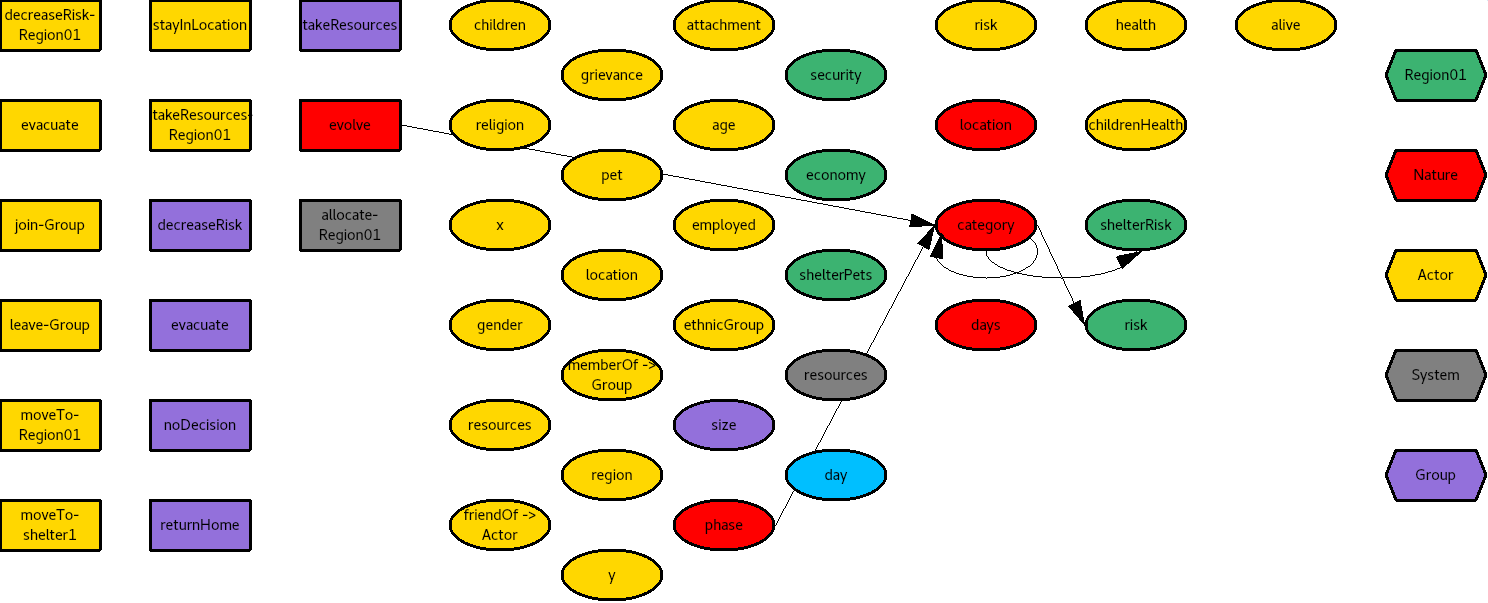
\includegraphics[width=0.8\textwidth]{images/categoryOfNature.png}%
\caption{Ground Truth subgraph for Nature's category}%
\end{figure}

%
\subsubsection{Effect of Nature{-}evolve on Nature's category}%
\label{ssubsec:Effect of Nature{-}evolve on Nature's category}%
\begin{flushleft}%
IF %
$\mbox{\textbf{Nature's phase}} '$%
$=$%
\textbf{none}%
 or %
\textbf{approaching}%
 or %
\textbf{active}%
\linebreak%
\hspace*{2em}%
IF %
\textbf{Nature's category}%
$=$%
0%
\linebreak%
\hspace*{4em}%
THEN %
\linebreak%
\hspace*{6em}%
20\%: %
$\mbox{\textbf{Nature's category}} '$%
$\leftarrow$%
1%
\linebreak%
\hspace*{6em}%
20\%: %
$\mbox{\textbf{Nature's category}} '$%
$\leftarrow$%
2%
\linebreak%
\hspace*{6em}%
20\%: %
$\mbox{\textbf{Nature's category}} '$%
$\leftarrow$%
3%
\linebreak%
\hspace*{6em}%
20\%: %
$\mbox{\textbf{Nature's category}} '$%
$\leftarrow$%
4%
\linebreak%
\hspace*{6em}%
20\%: %
$\mbox{\textbf{Nature's category}} '$%
$\leftarrow$%
5%
\linebreak%
\hspace*{4em}%
ELSE %
IF %
\textbf{Nature's category}%
$=$%
1%
\linebreak%
\hspace*{6em}%
THEN %
\linebreak%
\hspace*{8em}%
60\%: %
$\mbox{\textbf{Nature's category}} '$%
$\leftarrow$%
\textbf{Nature's category}%
\linebreak%
\hspace*{8em}%
40\%: %
$\mbox{\textbf{Nature's category}} '$%
$\leftarrow$%
2%
\linebreak%
\hspace*{6em}%
ELSE %
IF %
\textbf{Nature's category}%
$=$%
5%
\linebreak%
\hspace*{8em}%
THEN %
\linebreak%
\hspace*{10em}%
40\%: %
$\mbox{\textbf{Nature's category}} '$%
$\leftarrow$%
4%
\linebreak%
\hspace*{10em}%
60\%: %
$\mbox{\textbf{Nature's category}} '$%
$\leftarrow$%
\textbf{Nature's category}%
\linebreak%
\hspace*{8em}%
ELSE %
\linebreak%
\hspace*{10em}%
20\%: %
$\mbox{\textbf{Nature's category}} '$%
$\leftarrow$%
\textbf{Nature's category}%
${-}1$%
\linebreak%
\hspace*{10em}%
60\%: %
$\mbox{\textbf{Nature's category}} '$%
$\leftarrow$%
\textbf{Nature's category}%
\linebreak%
\hspace*{10em}%
20\%: %
$\mbox{\textbf{Nature's category}} '$%
$\leftarrow$%
\textbf{Nature's category}%
+1%
\linebreak%
\hspace*{2em}%
1 %
$\mbox{\textbf{Nature's category}} '$%
$\leftarrow$%
\textbf{Nature's category}%
\linebreak%
\hspace*{2em}%
2 %
$\mbox{\textbf{Nature's category}} '$%
$\leftarrow$%
0%
\end{flushleft}

%
\subsection{Nature's days}%
\label{subsec:Nature's days}%
\begin{description}%
\item[Type:]%
Integer%
\end{description}%


\begin{figure}[ht]%
\centering%
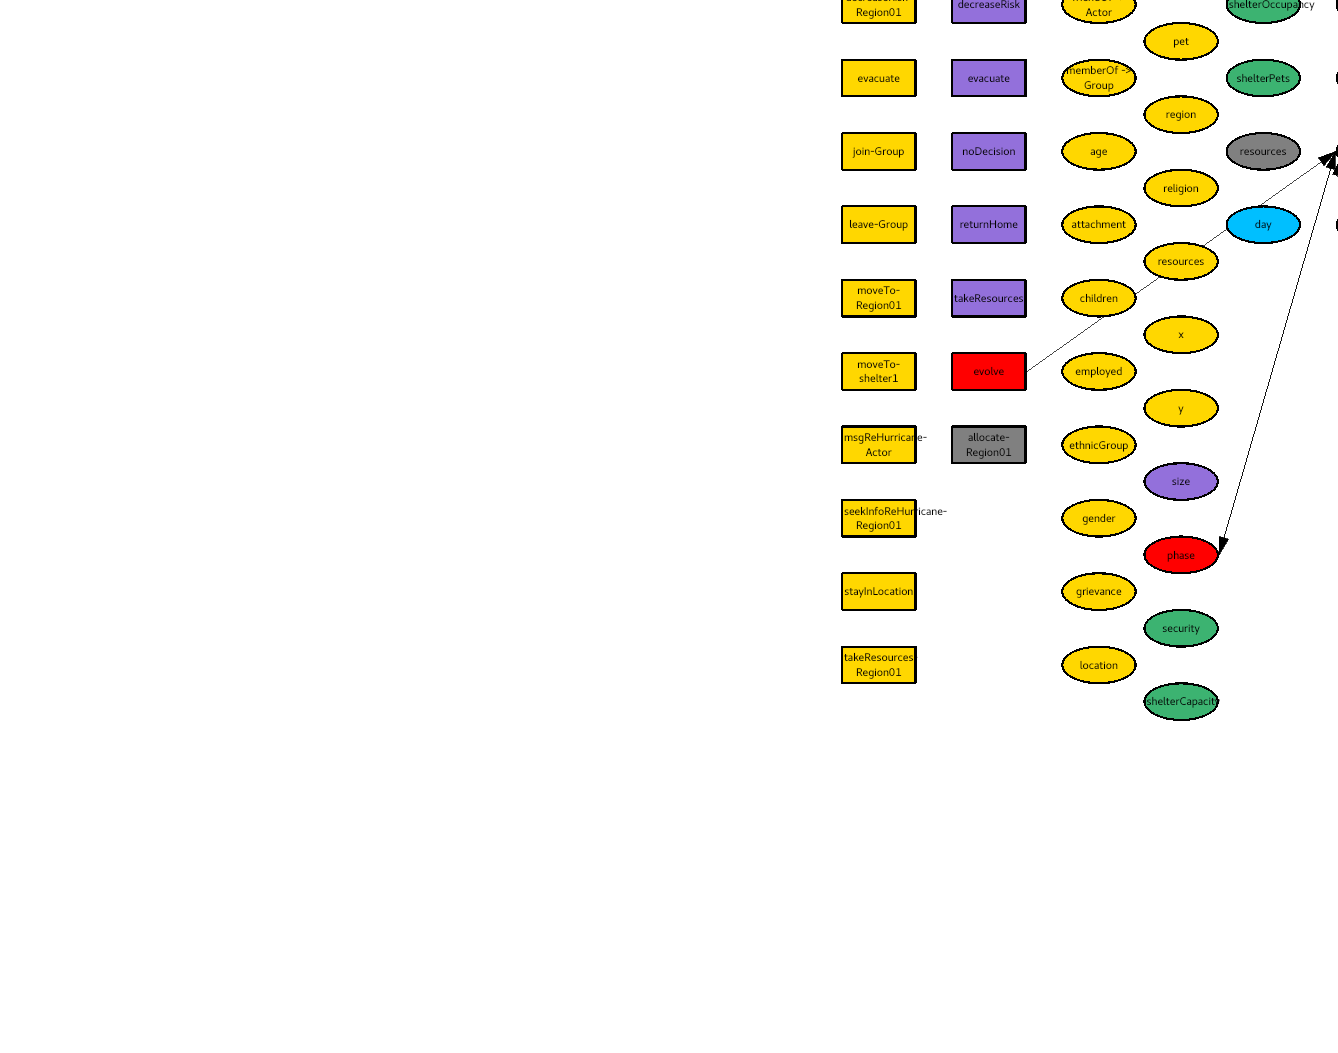
\includegraphics[width=0.8\textwidth]{images/daysOfNature.png}%
\caption{Ground Truth subgraph for Nature's days}%
\end{figure}

%
\subsubsection{Effect of Nature{-}evolve on Nature's days}%
\label{ssubsec:Effect of Nature{-}evolve on Nature's days}%
\begin{flushleft}%
IF %
\textbf{Nature's phase}%
$=$%
$\mbox{\textbf{Nature's phase}} '$%
\linebreak%
\hspace*{2em}%
THEN %
$\mbox{\textbf{Nature's days}} '$%
$\leftarrow$%
\textbf{Nature's days}%
+1%
\linebreak%
\hspace*{2em}%
ELSE %
$\mbox{\textbf{Nature's days}} '$%
$\leftarrow$%
0%
\end{flushleft}

%
\subsection{Nature's location}%
\label{subsec:Nature's location}%
\begin{description}%
\item[Type:]%
String%
\item[Values:]%
\textbf{Region01}%
, %
\textbf{none}%
\end{description}%


\begin{figure}[ht]%
\centering%
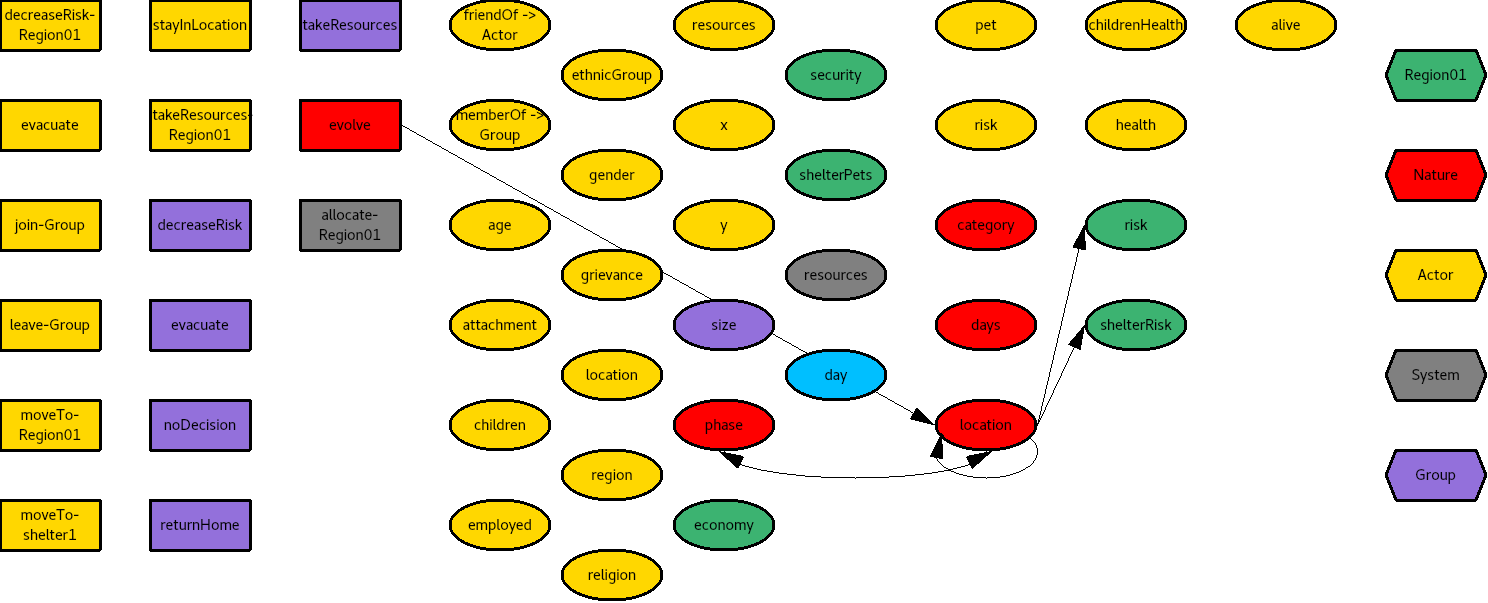
\includegraphics[width=0.8\textwidth]{images/locationOfNature.png}%
\caption{Ground Truth subgraph for Nature's location}%
\end{figure}

%
\subsubsection{Effect of Nature{-}evolve on Nature's location}%
\label{ssubsec:Effect of Nature{-}evolve on Nature's location}%
\begin{flushleft}%
IF %
$\mbox{\textbf{Nature's phase}} '$%
$=$%
\textbf{none}%
 or %
\textbf{approaching}%
 or %
\textbf{active}%
\linebreak%
\hspace*{2em}%
IF %
\textbf{Nature's location}%
$=$%
\textbf{none}%
\linebreak%
\hspace*{4em}%
THEN %
$\mbox{\textbf{Nature's location}} '$%
$\leftarrow$%
\textbf{Region01}%
\linebreak%
\hspace*{4em}%
ELSE %
$\mbox{\textbf{Nature's location}} '$%
$\leftarrow$%
\textbf{Nature's location}%
\linebreak%
\hspace*{2em}%
1 %
IF %
\textbf{Nature's location}%
$=$%
\textbf{Region01}%
\linebreak%
\hspace*{4em}%
$\mbox{\textbf{Nature's location}} '$%
$\leftarrow$%
\textbf{Nature's location}%
\linebreak%
\hspace*{4em}%
$\mbox{\textbf{Nature's location}} '$%
$\leftarrow$%
\textbf{none}%
\linebreak%
\hspace*{2em}%
2 %
$\mbox{\textbf{Nature's location}} '$%
$\leftarrow$%
\textbf{none}%
\end{flushleft}

%
\subsection{Nature's phase}%
\label{subsec:Nature's phase}%
\begin{description}%
\item[Type:]%
String%
\item[Values:]%
\textbf{active}%
, %
\textbf{approaching}%
, %
\textbf{none}%
\end{description}%


\begin{figure}[ht]%
\centering%
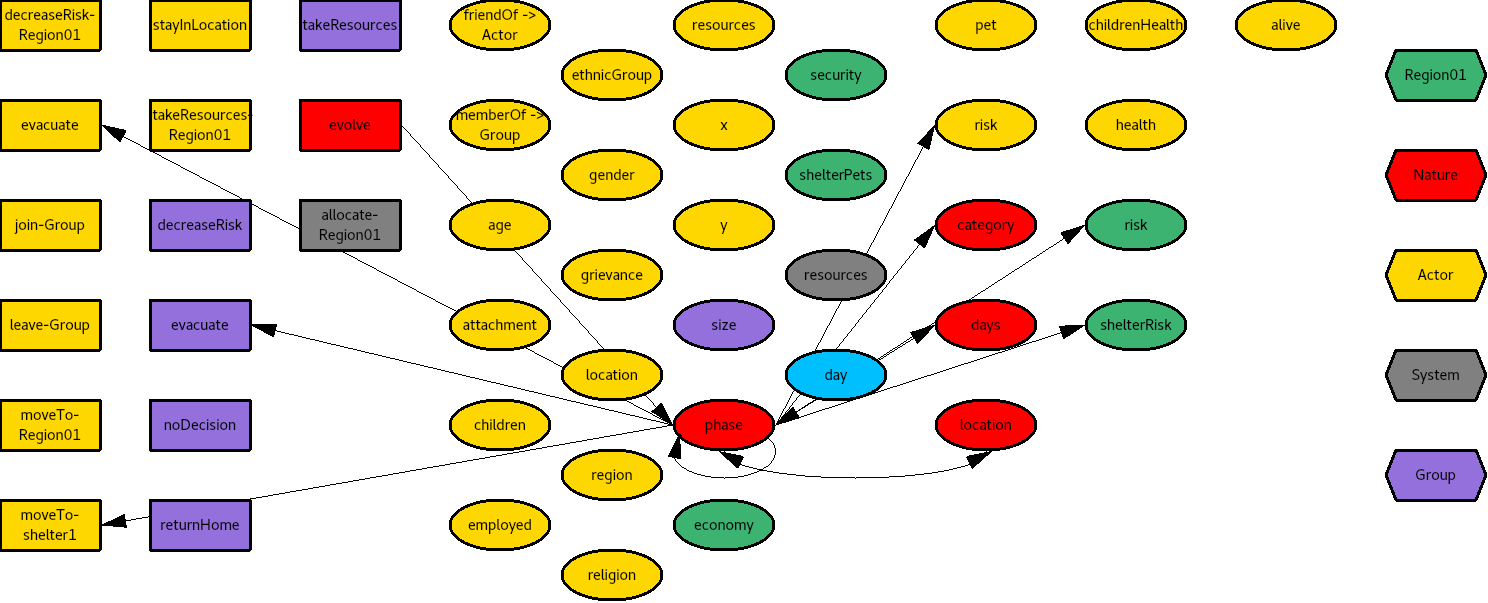
\includegraphics[width=0.8\textwidth]{images/phaseOfNature.png}%
\caption{Ground Truth subgraph for Nature's phase}%
\end{figure}

%
\subsubsection{Effect of Nature{-}evolve on Nature's phase}%
\label{ssubsec:Effect of Nature{-}evolve on Nature's phase}%
\begin{flushleft}%
IF %
\textbf{Nature's phase}%
$=$%
\textbf{none}%
 or %
\textbf{approaching}%
\linebreak%
\hspace*{2em}%
IF %
\textbf{Nature's days}%
$>$%
1%
\linebreak%
\hspace*{4em}%
THEN %
\linebreak%
\hspace*{6em}%
80\%: %
$\mbox{\textbf{Nature's phase}} '$%
$\leftarrow$%
\textbf{approaching}%
\linebreak%
\hspace*{6em}%
19\%: %
$\mbox{\textbf{Nature's phase}} '$%
$\leftarrow$%
\textbf{none}%
\linebreak%
\hspace*{4em}%
ELSE %
$\mbox{\textbf{Nature's phase}} '$%
$\leftarrow$%
\textbf{none}%
\linebreak%
\hspace*{2em}%
1 %
IF %
\textbf{Nature's days}%
$>$%
1%
\linebreak%
\hspace*{4em}%
THEN %
\linebreak%
\hspace*{6em}%
80\%: %
$\mbox{\textbf{Nature's phase}} '$%
$\leftarrow$%
\textbf{active}%
\linebreak%
\hspace*{6em}%
19\%: %
$\mbox{\textbf{Nature's phase}} '$%
$\leftarrow$%
\textbf{approaching}%
\linebreak%
\hspace*{4em}%
ELSE %
$\mbox{\textbf{Nature's phase}} '$%
$\leftarrow$%
\textbf{approaching}%
\linebreak%
\hspace*{2em}%
IF %
\textbf{Nature's location}%
$=$%
\textbf{none}%
\linebreak%
\hspace*{4em}%
THEN %
$\mbox{\textbf{Nature's phase}} '$%
$\leftarrow$%
\textbf{none}%
\linebreak%
\hspace*{4em}%
ELSE %
$\mbox{\textbf{Nature's phase}} '$%
$\leftarrow$%
\textbf{active}%
\end{flushleft}

%
\subsection{Region01's economy}%
\label{subsec:Region01's economy}%
Current economic level of region%
\begin{description}%
\item[Type:]%
Real%
\end{description}

%
\subsection{Region01's risk}%
\label{subsec:Region01's risk}%
Level of risk from hurricane%
\begin{description}%
\item[Type:]%
Real%
\end{description}%


\begin{figure}[ht]%
\centering%
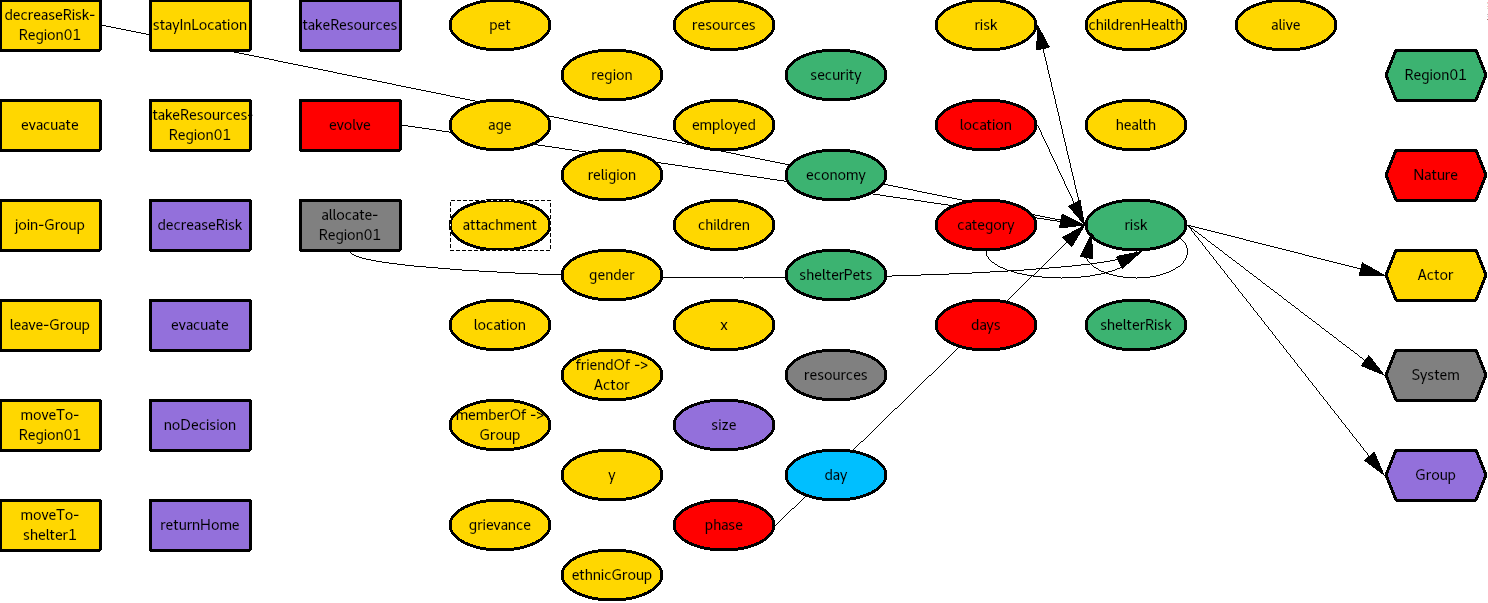
\includegraphics[width=0.8\textwidth]{images/riskOfRegion01.png}%
\caption{Ground Truth subgraph for Region01's risk}%
\end{figure}

%
\subsubsection{Effect of Actor{-}decreaseRisk{-}Region01 on Region01's risk}%
\label{ssubsec:Effect of Actor{-}decreaseRisk{-}Region01 on Region01's risk}%
\begin{flushleft}%
$\mbox{\textbf{Region01's risk}} '$%
$\leftarrow$%
80\%%
$\cdot$%
\textbf{Region01's risk}%
\end{flushleft}

%
\subsubsection{Effect of Nature{-}evolve on Region01's risk}%
\label{ssubsec:Effect of Nature{-}evolve on Region01's risk}%
\begin{flushleft}%
IF %
$\mbox{\textbf{Nature's phase}} '$%
$=$%
\textbf{active}%
\linebreak%
\hspace*{2em}%
THEN %
IF %
$\mbox{\textbf{Nature's location}} '$%
$=$%
\textbf{Region01}%
\linebreak%
\hspace*{4em}%
$\mbox{\textbf{Region01's risk}} '$%
$\leftarrow$%
80\%%
$\cdot$%
\textbf{Region01's risk}%
\linebreak%
\hspace*{4em}%
IF %
\textbf{Nature's category}%
$=$%
{[}1,2,3,4,5{]}%
\linebreak%
\hspace*{6em}%
$\mbox{\textbf{Region01's risk}} '$%
$\leftarrow$%
90\%%
$\cdot$%
\textbf{Region01's risk}%
+0.10%
\linebreak%
\hspace*{6em}%
1 %
$\mbox{\textbf{Region01's risk}} '$%
$\leftarrow$%
80\%%
$\cdot$%
\textbf{Region01's risk}%
+0.20%
\linebreak%
\hspace*{6em}%
2 %
$\mbox{\textbf{Region01's risk}} '$%
$\leftarrow$%
70\%%
$\cdot$%
\textbf{Region01's risk}%
+0.30%
\linebreak%
\hspace*{6em}%
3 %
$\mbox{\textbf{Region01's risk}} '$%
$\leftarrow$%
60\%%
$\cdot$%
\textbf{Region01's risk}%
+0.40%
\linebreak%
\hspace*{6em}%
4 %
$\mbox{\textbf{Region01's risk}} '$%
$\leftarrow$%
50\%%
$\cdot$%
\textbf{Region01's risk}%
+0.50%
\linebreak%
\hspace*{2em}%
ELSE %
$\mbox{\textbf{Region01's risk}} '$%
$\leftarrow$%
80\%%
$\cdot$%
\textbf{Region01's risk}%
\end{flushleft}

%
\subsubsection{Effect of System{-}allocate{-}Region01 on Region01's risk}%
\label{ssubsec:Effect of System{-}allocate{-}Region01 on Region01's risk}%
\begin{flushleft}%
$\mbox{\textbf{Region01's risk}} '$%
$\leftarrow$%
80\%%
$\cdot$%
\textbf{Region01's risk}%
\end{flushleft}

%
\subsection{Region01's security}%
\label{subsec:Region01's security}%
Level of law enforcement in region%
\begin{description}%
\item[Type:]%
Real%
\end{description}

%
\subsection{Region01's shelterPets}%
\label{subsec:Region01's shelterPets}%
\begin{description}%
\item[Type:]%
Boolean%
\end{description}

%
\subsection{Region01's shelterRisk}%
\label{subsec:Region01's shelterRisk}%
\begin{description}%
\item[Type:]%
Real%
\end{description}%


\begin{figure}[ht]%
\centering%
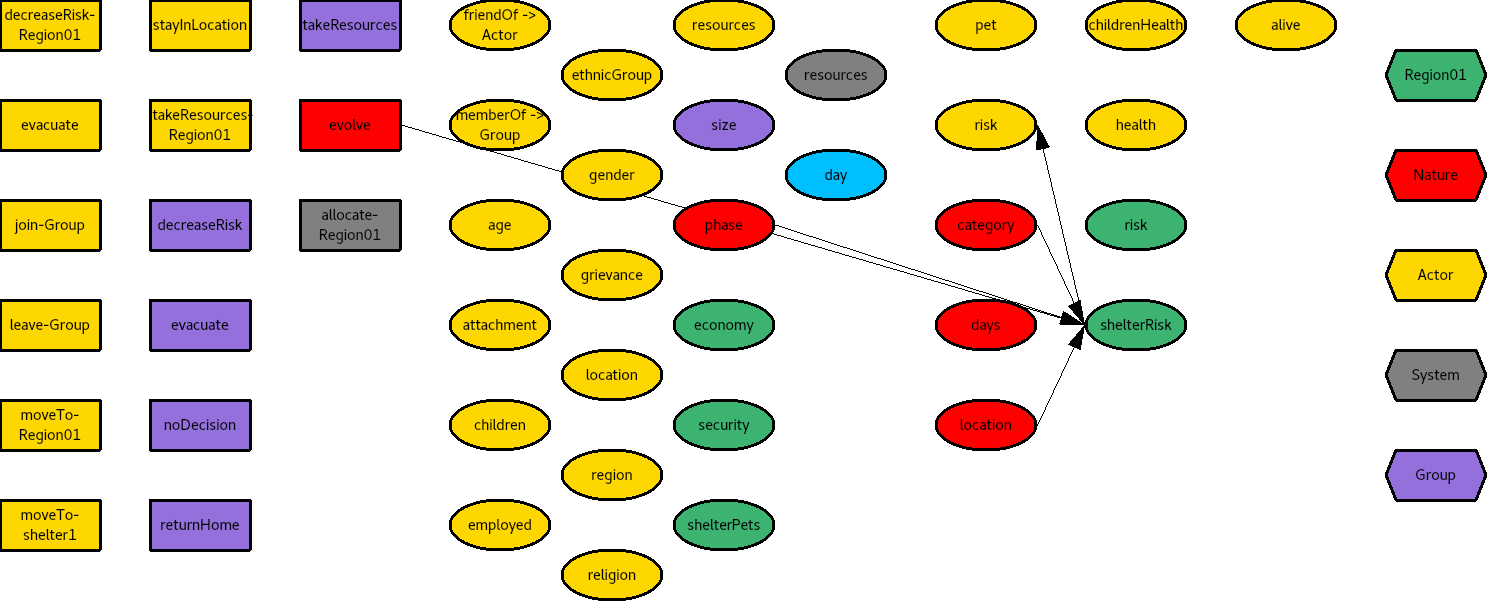
\includegraphics[width=0.8\textwidth]{images/shelterRiskOfRegion01.png}%
\caption{Ground Truth subgraph for Region01's shelterRisk}%
\end{figure}

%
\subsubsection{Effect of Nature{-}evolve on Region01's shelterRisk}%
\label{ssubsec:Effect of Nature{-}evolve on Region01's shelterRisk}%
\begin{flushleft}%
IF %
$\mbox{\textbf{Nature's phase}} '$%
$=$%
\textbf{active}%
\linebreak%
\hspace*{2em}%
THEN %
IF %
$\mbox{\textbf{Nature's location}} '$%
$=$%
\textbf{Region01}%
\linebreak%
\hspace*{4em}%
THEN %
IF %
\textbf{Nature's category}%
$=$%
{[}1,2,3,4,5{]}%
\linebreak%
\hspace*{6em}%
$\mbox{\textbf{Region01's shelterRisk}} '$%
$\leftarrow$%
\textbf{Region01's shelterRisk}%
\linebreak%
\hspace*{6em}%
1 %
$\mbox{\textbf{Region01's shelterRisk}} '$%
$\leftarrow$%
80\%%
$\cdot$%
\textbf{Region01's shelterRisk}%
+0.20%
\linebreak%
\hspace*{6em}%
2 %
$\mbox{\textbf{Region01's shelterRisk}} '$%
$\leftarrow$%
60\%%
$\cdot$%
\textbf{Region01's shelterRisk}%
+0.40%
\linebreak%
\hspace*{6em}%
3 %
$\mbox{\textbf{Region01's shelterRisk}} '$%
$\leftarrow$%
39\%%
$\cdot$%
\textbf{Region01's shelterRisk}%
+0.60%
\linebreak%
\hspace*{6em}%
4 %
$\mbox{\textbf{Region01's shelterRisk}} '$%
$\leftarrow$%
19\%%
$\cdot$%
\textbf{Region01's shelterRisk}%
+0.80%
\linebreak%
\hspace*{4em}%
ELSE %
$\mbox{\textbf{Region01's shelterRisk}} '$%
$\leftarrow$%
\textbf{Region01's shelterRisk}%
\linebreak%
\hspace*{2em}%
ELSE %
$\mbox{\textbf{Region01's shelterRisk}} '$%
$\leftarrow$%
80\%%
$\cdot$%
\textbf{Region01's shelterRisk}%
\end{flushleft}

%
\subsection{System's resources}%
\label{subsec:System's resources}%
\begin{description}%
\item[Type:]%
Integer%
\end{description}%


\begin{figure}[ht]%
\centering%
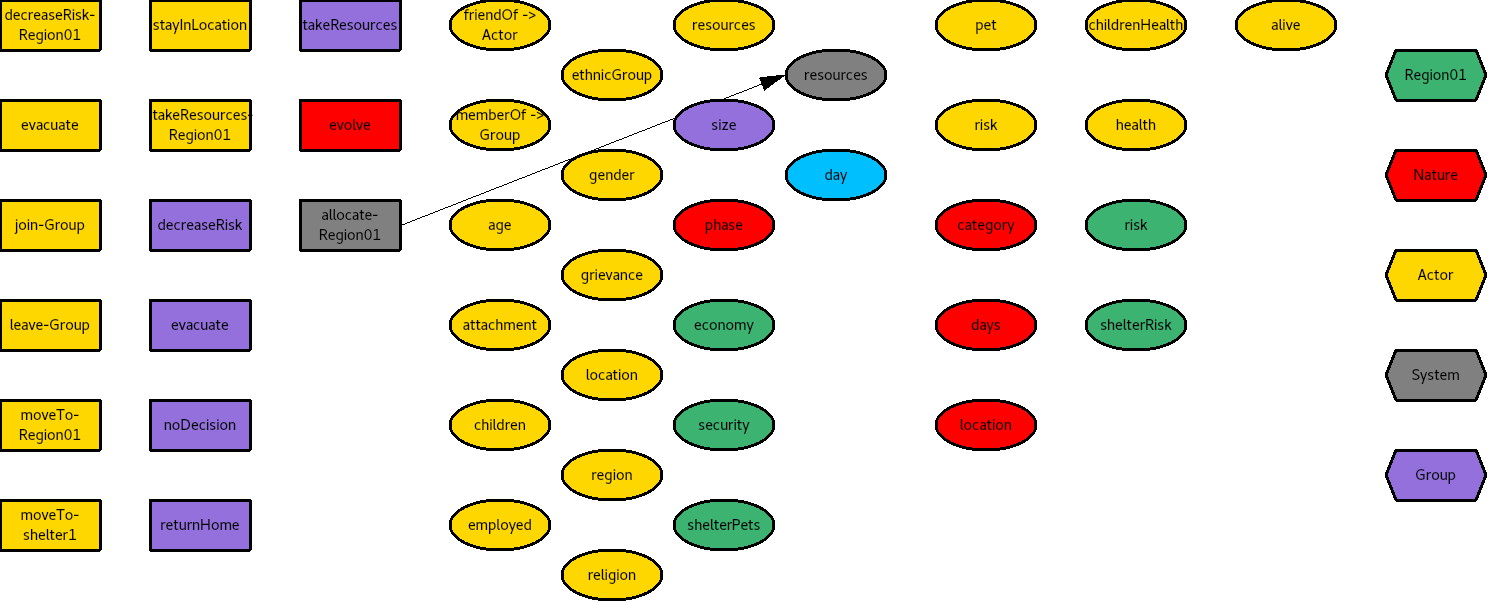
\includegraphics[width=0.8\textwidth]{images/resourcesOfSystem.png}%
\caption{Ground Truth subgraph for System's resources}%
\end{figure}

%
\subsection{day}%
\label{subsec:day}%
\begin{description}%
\item[Type:]%
Integer%
\end{description}%


\begin{figure}[ht]%
\centering%
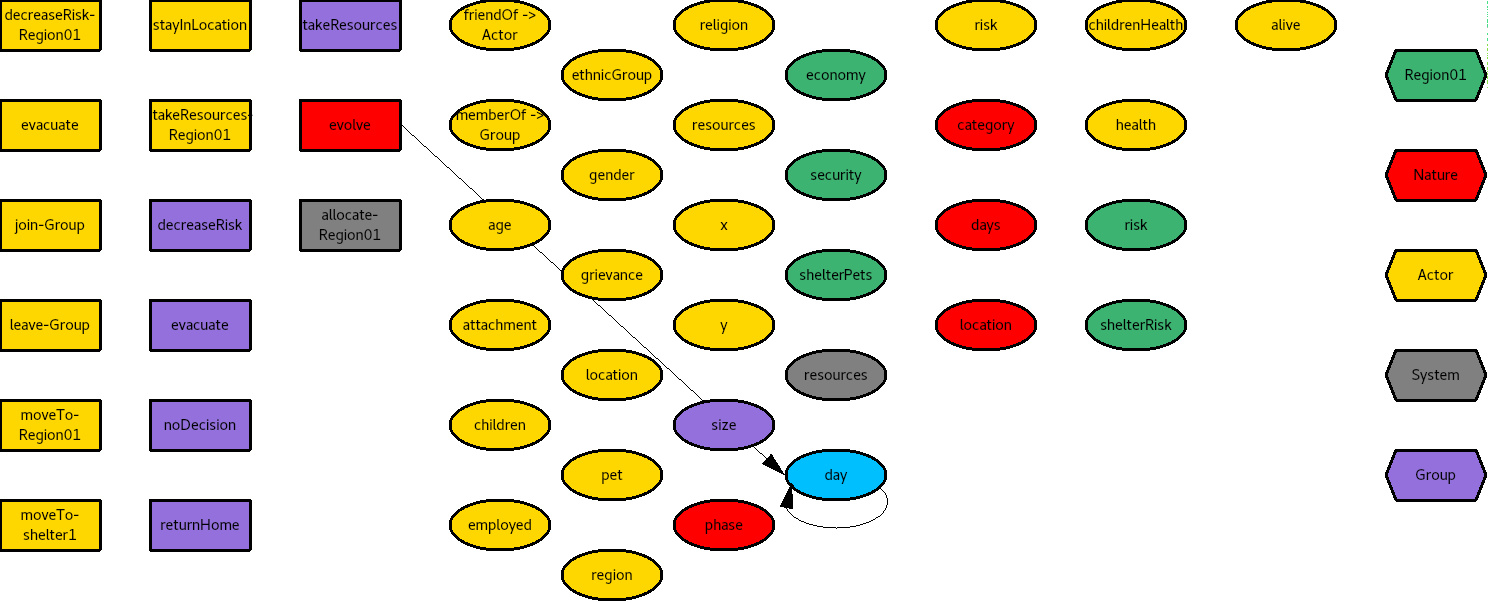
\includegraphics[width=0.8\textwidth]{images/day.png}%
\caption{Ground Truth subgraph for day}%
\end{figure}

%
\subsubsection{Effect of Nature{-}evolve on day}%
\label{ssubsec:Effect of Nature{-}evolve on day}%
\begin{flushleft}%
$\mbox{\textbf{day}} '$%
$\leftarrow$%
\textbf{day}%
+1%
\end{flushleft}

%
\section{Relations}%
\label{sec:Relations}%
\subsection{Actor friendOf Actor}%
\label{subsec:Actor friendOf Actor}%
\begin{description}%
\item[Type:]%
Boolean%
\end{description}

%
\subsection{Actor memberOf Group}%
\label{subsec:Actor memberOf Group}%
\begin{description}%
\item[Type:]%
Boolean%
\end{description}%


\begin{figure}[ht]%
\centering%
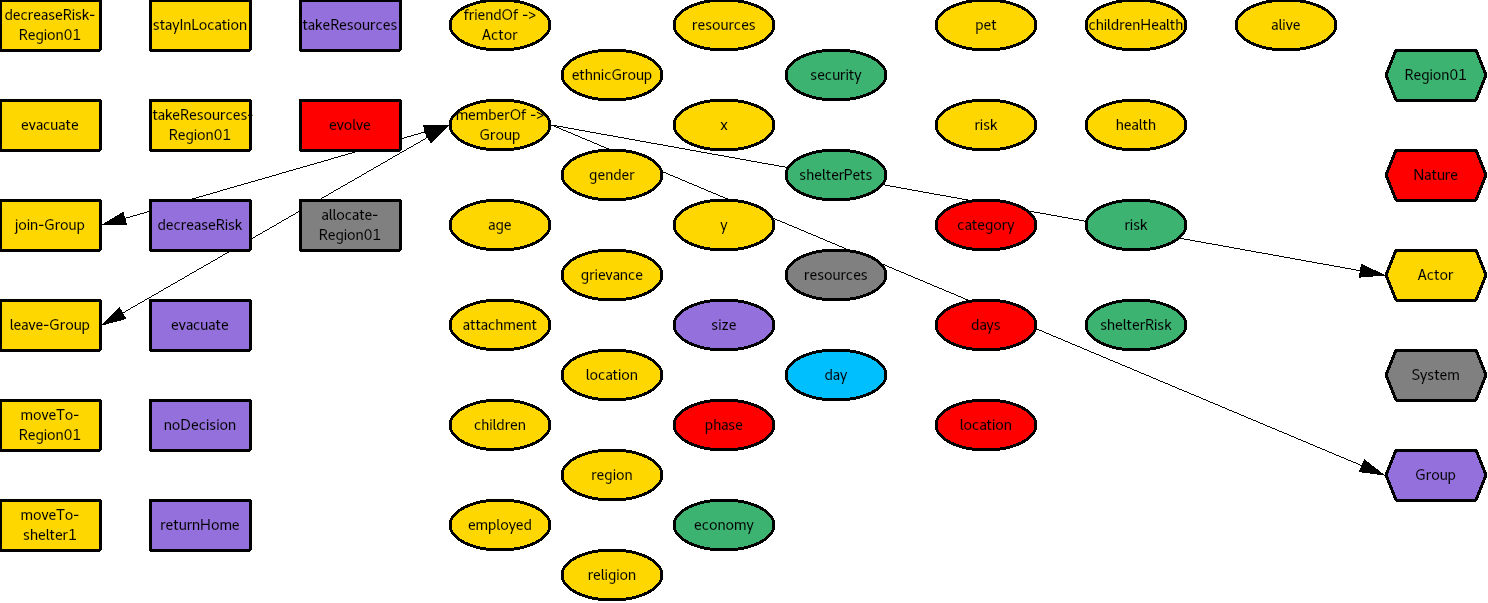
\includegraphics[width=0.8\textwidth]{images/ActormemberOf->Group.png}%
\caption{Ground Truth subgraph for Actor memberOf {-}> Group}%
\end{figure}

%
\subsubsection{Effect of Actor{-}join{-}Group on Actor memberOf Group}%
\label{ssubsec:Effect of Actor{-}join{-}Group on Actor memberOf Group}%
\begin{flushleft}%
$\mbox{\textbf{Actor memberOf Group}} '$%
$\leftarrow$%
\textbf{true}%
\end{flushleft}

%
\subsubsection{Effect of Actor{-}leave{-}Group on Actor memberOf Group}%
\label{ssubsec:Effect of Actor{-}leave{-}Group on Actor memberOf Group}%
\begin{flushleft}%
$\mbox{\textbf{Actor memberOf Group}} '$%
$\leftarrow$%
\textbf{false}%
\end{flushleft}

%
\section{Actions}%
\label{sec:Actions}%
\subsection{Nature evolve}%
\label{subsec:Nature evolve}%


\begin{figure}[ht]%
\centering%
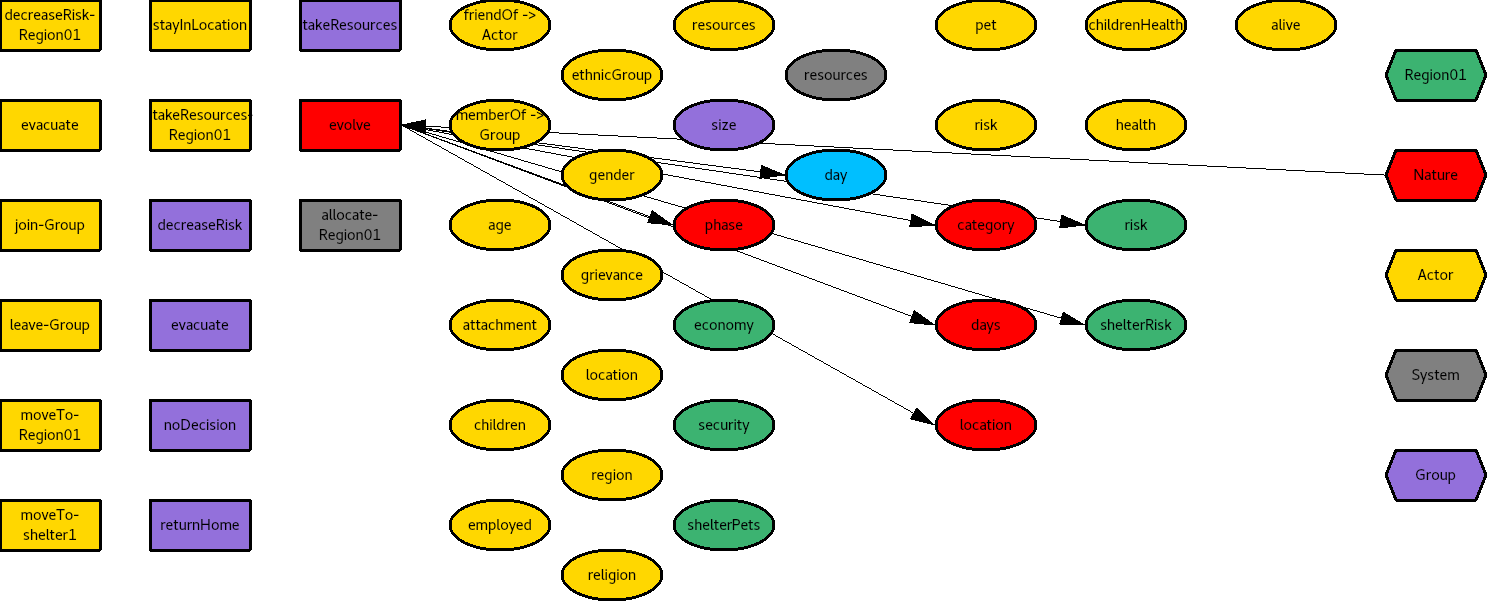
\includegraphics[width=0.8\textwidth]{images/Nature-evolve.png}%
\caption{Ground Truth subgraph for Nature{-}evolve}%
\end{figure}

%
\subsubsection{Effect on Nature's category of Nature evolve}%
\label{ssubsec:Effect on Nature's category of Nature evolve}%
\begin{flushleft}%
IF %
$\mbox{\textbf{Nature's phase}} '$%
$=$%
\textbf{none}%
 or %
\textbf{approaching}%
 or %
\textbf{active}%
\linebreak%
\hspace*{2em}%
IF %
\textbf{Nature's category}%
$=$%
0%
\linebreak%
\hspace*{4em}%
THEN %
\linebreak%
\hspace*{6em}%
20\%: %
$\mbox{\textbf{Nature's category}} '$%
$\leftarrow$%
1%
\linebreak%
\hspace*{6em}%
20\%: %
$\mbox{\textbf{Nature's category}} '$%
$\leftarrow$%
2%
\linebreak%
\hspace*{6em}%
20\%: %
$\mbox{\textbf{Nature's category}} '$%
$\leftarrow$%
3%
\linebreak%
\hspace*{6em}%
20\%: %
$\mbox{\textbf{Nature's category}} '$%
$\leftarrow$%
4%
\linebreak%
\hspace*{6em}%
20\%: %
$\mbox{\textbf{Nature's category}} '$%
$\leftarrow$%
5%
\linebreak%
\hspace*{4em}%
ELSE %
IF %
\textbf{Nature's category}%
$=$%
1%
\linebreak%
\hspace*{6em}%
THEN %
\linebreak%
\hspace*{8em}%
60\%: %
$\mbox{\textbf{Nature's category}} '$%
$\leftarrow$%
\textbf{Nature's category}%
\linebreak%
\hspace*{8em}%
40\%: %
$\mbox{\textbf{Nature's category}} '$%
$\leftarrow$%
2%
\linebreak%
\hspace*{6em}%
ELSE %
IF %
\textbf{Nature's category}%
$=$%
5%
\linebreak%
\hspace*{8em}%
THEN %
\linebreak%
\hspace*{10em}%
40\%: %
$\mbox{\textbf{Nature's category}} '$%
$\leftarrow$%
4%
\linebreak%
\hspace*{10em}%
60\%: %
$\mbox{\textbf{Nature's category}} '$%
$\leftarrow$%
\textbf{Nature's category}%
\linebreak%
\hspace*{8em}%
ELSE %
\linebreak%
\hspace*{10em}%
20\%: %
$\mbox{\textbf{Nature's category}} '$%
$\leftarrow$%
\textbf{Nature's category}%
${-}1$%
\linebreak%
\hspace*{10em}%
60\%: %
$\mbox{\textbf{Nature's category}} '$%
$\leftarrow$%
\textbf{Nature's category}%
\linebreak%
\hspace*{10em}%
20\%: %
$\mbox{\textbf{Nature's category}} '$%
$\leftarrow$%
\textbf{Nature's category}%
+1%
\linebreak%
\hspace*{2em}%
1 %
$\mbox{\textbf{Nature's category}} '$%
$\leftarrow$%
\textbf{Nature's category}%
\linebreak%
\hspace*{2em}%
2 %
$\mbox{\textbf{Nature's category}} '$%
$\leftarrow$%
0%
\end{flushleft}

%
\subsubsection{Effect on Nature's days of Nature evolve}%
\label{ssubsec:Effect on Nature's days of Nature evolve}%
\begin{flushleft}%
IF %
\textbf{Nature's phase}%
$=$%
$\mbox{\textbf{Nature's phase}} '$%
\linebreak%
\hspace*{2em}%
THEN %
$\mbox{\textbf{Nature's days}} '$%
$\leftarrow$%
\textbf{Nature's days}%
+1%
\linebreak%
\hspace*{2em}%
ELSE %
$\mbox{\textbf{Nature's days}} '$%
$\leftarrow$%
0%
\end{flushleft}

%
\subsubsection{Effect on Nature's location of Nature evolve}%
\label{ssubsec:Effect on Nature's location of Nature evolve}%
\begin{flushleft}%
IF %
$\mbox{\textbf{Nature's phase}} '$%
$=$%
\textbf{none}%
 or %
\textbf{approaching}%
 or %
\textbf{active}%
\linebreak%
\hspace*{2em}%
IF %
\textbf{Nature's location}%
$=$%
\textbf{none}%
\linebreak%
\hspace*{4em}%
THEN %
$\mbox{\textbf{Nature's location}} '$%
$\leftarrow$%
\textbf{Region01}%
\linebreak%
\hspace*{4em}%
ELSE %
$\mbox{\textbf{Nature's location}} '$%
$\leftarrow$%
\textbf{Nature's location}%
\linebreak%
\hspace*{2em}%
1 %
IF %
\textbf{Nature's location}%
$=$%
\textbf{Region01}%
\linebreak%
\hspace*{4em}%
$\mbox{\textbf{Nature's location}} '$%
$\leftarrow$%
\textbf{Nature's location}%
\linebreak%
\hspace*{4em}%
$\mbox{\textbf{Nature's location}} '$%
$\leftarrow$%
\textbf{none}%
\linebreak%
\hspace*{2em}%
2 %
$\mbox{\textbf{Nature's location}} '$%
$\leftarrow$%
\textbf{none}%
\end{flushleft}

%
\subsubsection{Effect on Nature's phase of Nature evolve}%
\label{ssubsec:Effect on Nature's phase of Nature evolve}%
\begin{flushleft}%
IF %
\textbf{Nature's phase}%
$=$%
\textbf{none}%
 or %
\textbf{approaching}%
\linebreak%
\hspace*{2em}%
IF %
\textbf{Nature's days}%
$>$%
1%
\linebreak%
\hspace*{4em}%
THEN %
\linebreak%
\hspace*{6em}%
80\%: %
$\mbox{\textbf{Nature's phase}} '$%
$\leftarrow$%
\textbf{approaching}%
\linebreak%
\hspace*{6em}%
19\%: %
$\mbox{\textbf{Nature's phase}} '$%
$\leftarrow$%
\textbf{none}%
\linebreak%
\hspace*{4em}%
ELSE %
$\mbox{\textbf{Nature's phase}} '$%
$\leftarrow$%
\textbf{none}%
\linebreak%
\hspace*{2em}%
1 %
IF %
\textbf{Nature's days}%
$>$%
1%
\linebreak%
\hspace*{4em}%
THEN %
\linebreak%
\hspace*{6em}%
80\%: %
$\mbox{\textbf{Nature's phase}} '$%
$\leftarrow$%
\textbf{active}%
\linebreak%
\hspace*{6em}%
19\%: %
$\mbox{\textbf{Nature's phase}} '$%
$\leftarrow$%
\textbf{approaching}%
\linebreak%
\hspace*{4em}%
ELSE %
$\mbox{\textbf{Nature's phase}} '$%
$\leftarrow$%
\textbf{approaching}%
\linebreak%
\hspace*{2em}%
IF %
\textbf{Nature's location}%
$=$%
\textbf{none}%
\linebreak%
\hspace*{4em}%
THEN %
$\mbox{\textbf{Nature's phase}} '$%
$\leftarrow$%
\textbf{none}%
\linebreak%
\hspace*{4em}%
ELSE %
$\mbox{\textbf{Nature's phase}} '$%
$\leftarrow$%
\textbf{active}%
\end{flushleft}

%
\subsubsection{Effect on Region01's risk of Nature evolve}%
\label{ssubsec:Effect on Region01's risk of Nature evolve}%
\begin{flushleft}%
IF %
$\mbox{\textbf{Nature's phase}} '$%
$=$%
\textbf{active}%
\linebreak%
\hspace*{2em}%
THEN %
IF %
$\mbox{\textbf{Nature's location}} '$%
$=$%
\textbf{Region01}%
\linebreak%
\hspace*{4em}%
$\mbox{\textbf{Region01's risk}} '$%
$\leftarrow$%
80\%%
$\cdot$%
\textbf{Region01's risk}%
\linebreak%
\hspace*{4em}%
IF %
\textbf{Nature's category}%
$=$%
{[}1,2,3,4,5{]}%
\linebreak%
\hspace*{6em}%
$\mbox{\textbf{Region01's risk}} '$%
$\leftarrow$%
90\%%
$\cdot$%
\textbf{Region01's risk}%
+0.10%
\linebreak%
\hspace*{6em}%
1 %
$\mbox{\textbf{Region01's risk}} '$%
$\leftarrow$%
80\%%
$\cdot$%
\textbf{Region01's risk}%
+0.20%
\linebreak%
\hspace*{6em}%
2 %
$\mbox{\textbf{Region01's risk}} '$%
$\leftarrow$%
70\%%
$\cdot$%
\textbf{Region01's risk}%
+0.30%
\linebreak%
\hspace*{6em}%
3 %
$\mbox{\textbf{Region01's risk}} '$%
$\leftarrow$%
60\%%
$\cdot$%
\textbf{Region01's risk}%
+0.40%
\linebreak%
\hspace*{6em}%
4 %
$\mbox{\textbf{Region01's risk}} '$%
$\leftarrow$%
50\%%
$\cdot$%
\textbf{Region01's risk}%
+0.50%
\linebreak%
\hspace*{2em}%
ELSE %
$\mbox{\textbf{Region01's risk}} '$%
$\leftarrow$%
80\%%
$\cdot$%
\textbf{Region01's risk}%
\end{flushleft}

%
\subsubsection{Effect on Region01's shelterRisk of Nature evolve}%
\label{ssubsec:Effect on Region01's shelterRisk of Nature evolve}%
\begin{flushleft}%
IF %
$\mbox{\textbf{Nature's phase}} '$%
$=$%
\textbf{active}%
\linebreak%
\hspace*{2em}%
THEN %
IF %
$\mbox{\textbf{Nature's location}} '$%
$=$%
\textbf{Region01}%
\linebreak%
\hspace*{4em}%
THEN %
IF %
\textbf{Nature's category}%
$=$%
{[}1,2,3,4,5{]}%
\linebreak%
\hspace*{6em}%
$\mbox{\textbf{Region01's shelterRisk}} '$%
$\leftarrow$%
\textbf{Region01's shelterRisk}%
\linebreak%
\hspace*{6em}%
1 %
$\mbox{\textbf{Region01's shelterRisk}} '$%
$\leftarrow$%
80\%%
$\cdot$%
\textbf{Region01's shelterRisk}%
+0.20%
\linebreak%
\hspace*{6em}%
2 %
$\mbox{\textbf{Region01's shelterRisk}} '$%
$\leftarrow$%
60\%%
$\cdot$%
\textbf{Region01's shelterRisk}%
+0.40%
\linebreak%
\hspace*{6em}%
3 %
$\mbox{\textbf{Region01's shelterRisk}} '$%
$\leftarrow$%
39\%%
$\cdot$%
\textbf{Region01's shelterRisk}%
+0.60%
\linebreak%
\hspace*{6em}%
4 %
$\mbox{\textbf{Region01's shelterRisk}} '$%
$\leftarrow$%
19\%%
$\cdot$%
\textbf{Region01's shelterRisk}%
+0.80%
\linebreak%
\hspace*{4em}%
ELSE %
$\mbox{\textbf{Region01's shelterRisk}} '$%
$\leftarrow$%
\textbf{Region01's shelterRisk}%
\linebreak%
\hspace*{2em}%
ELSE %
$\mbox{\textbf{Region01's shelterRisk}} '$%
$\leftarrow$%
80\%%
$\cdot$%
\textbf{Region01's shelterRisk}%
\end{flushleft}

%
\subsubsection{Effect on day of Nature evolve}%
\label{ssubsec:Effect on day of Nature evolve}%
\begin{flushleft}%
$\mbox{\textbf{day}} '$%
$\leftarrow$%
\textbf{day}%
+1%
\end{flushleft}

%
\subsection{Actor decreaseRisk Region01}%
\label{subsec:Actor decreaseRisk Region01}%


\begin{figure}[ht]%
\centering%
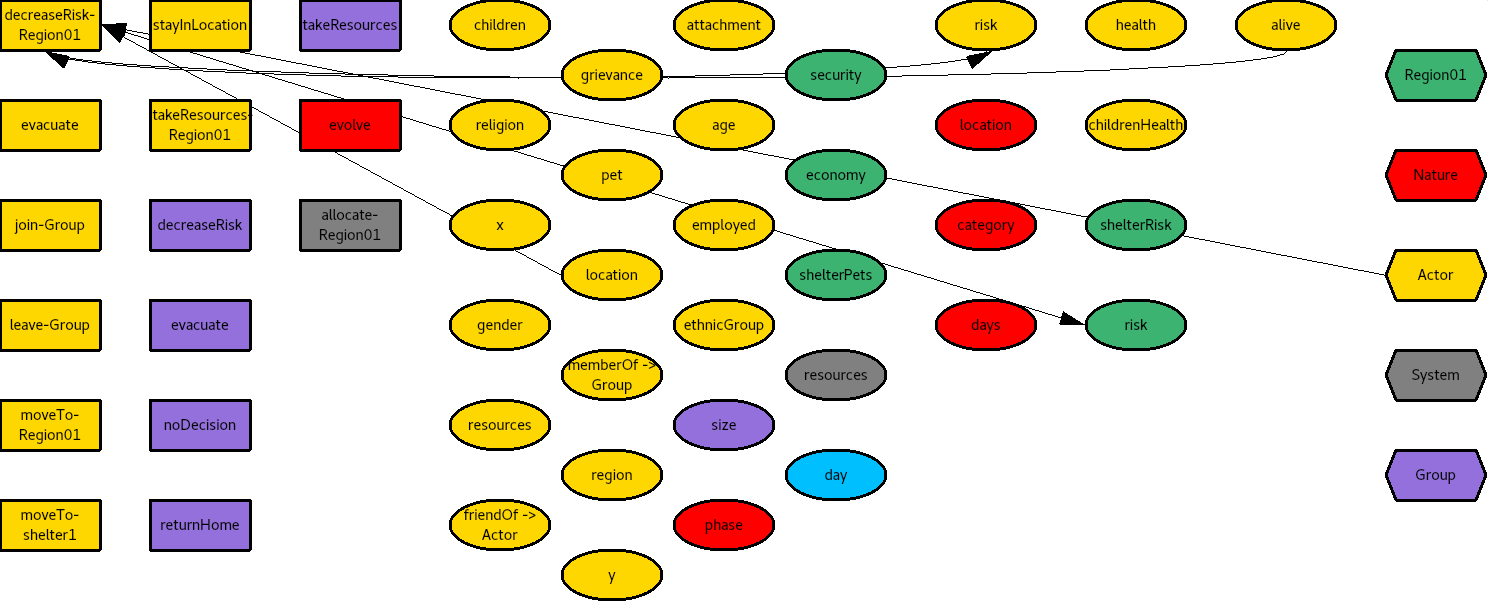
\includegraphics[width=0.8\textwidth]{images/Actor-decreaseRisk-Region01.png}%
\caption{Ground Truth subgraph for Actor{-}decreaseRisk{-}Region01}%
\end{figure}

%
\subsubsection{Applicability of Actor decreaseRisk Region01}%
\label{ssubsec:Applicability of Actor decreaseRisk Region01}%
\begin{flushleft}%
IF %
\textbf{Actor's location}%
$=$%
\textbf{Region01}%
\linebreak%
\hspace*{2em}%
THEN %
IF %
\textbf{Actor's alive}%
\linebreak%
\hspace*{4em}%
THEN %
\textbf{true}%
\linebreak%
\hspace*{4em}%
ELSE %
\textbf{false}%
\linebreak%
\hspace*{2em}%
ELSE %
\textbf{false}%
\end{flushleft}

%
\subsubsection{Effect on Actor's risk of Actor decreaseRisk Region01}%
\label{ssubsec:Effect on Actor's risk of Actor decreaseRisk Region01}%
\begin{flushleft}%
$\mbox{\textbf{Actor's risk}} '$%
$\leftarrow$%
80\%%
$\cdot$%
\textbf{Actor's risk}%
+0.20%
\end{flushleft}

%
\subsubsection{Effect on Region01's risk of Actor decreaseRisk Region01}%
\label{ssubsec:Effect on Region01's risk of Actor decreaseRisk Region01}%
\begin{flushleft}%
$\mbox{\textbf{Region01's risk}} '$%
$\leftarrow$%
80\%%
$\cdot$%
\textbf{Region01's risk}%
\end{flushleft}

%
\subsection{Actor evacuate}%
\label{subsec:Actor evacuate}%


\begin{figure}[ht]%
\centering%
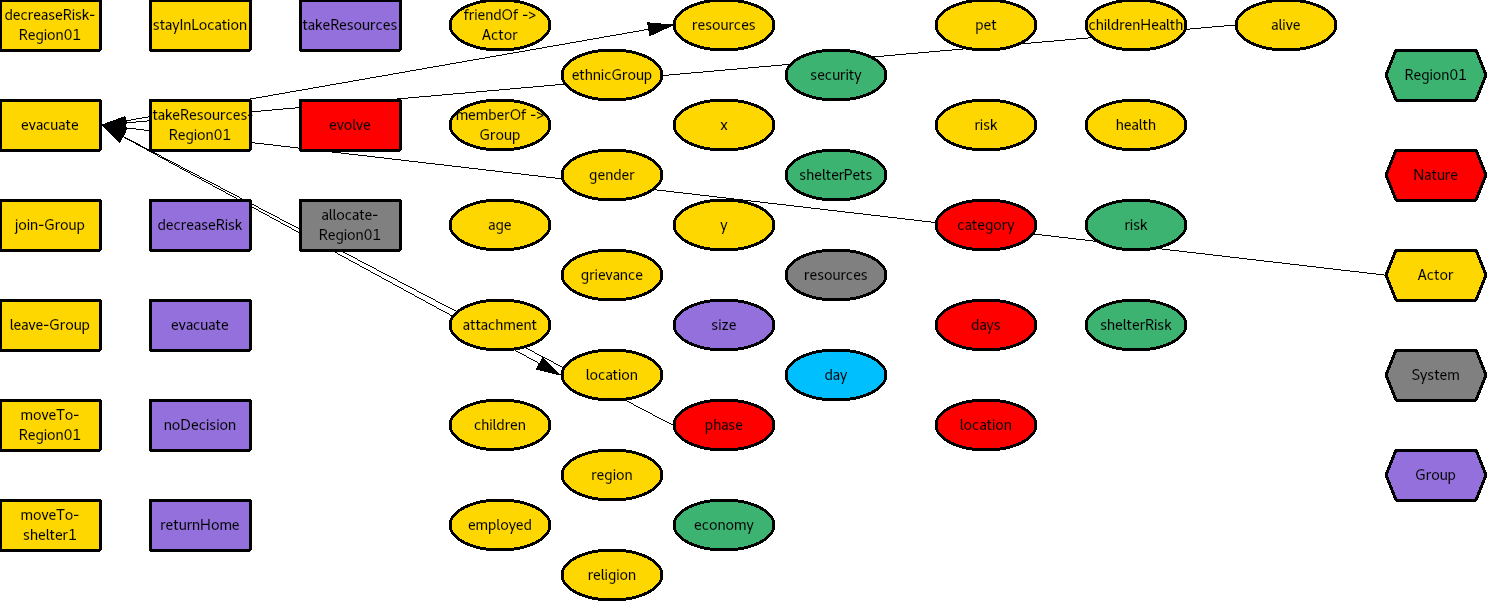
\includegraphics[width=0.8\textwidth]{images/Actor-evacuate.png}%
\caption{Ground Truth subgraph for Actor{-}evacuate}%
\end{figure}

%
\subsubsection{Applicability of Actor evacuate}%
\label{ssubsec:Applicability of Actor evacuate}%
\begin{flushleft}%
IF %
\textbf{Nature's phase}%
$=$%
\textbf{none}%
\linebreak%
\hspace*{2em}%
THEN %
\textbf{false}%
\linebreak%
\hspace*{2em}%
ELSE %
IF %
\textbf{Actor's location}%
$=$%
\textbf{evacuated}%
\linebreak%
\hspace*{4em}%
THEN %
\textbf{false}%
\linebreak%
\hspace*{4em}%
ELSE %
IF %
\textbf{Actor's alive}%
\linebreak%
\hspace*{6em}%
THEN %
\textbf{true}%
\linebreak%
\hspace*{6em}%
ELSE %
\textbf{false}%
\end{flushleft}

%
\subsubsection{Effect on Actor's location of Actor evacuate}%
\label{ssubsec:Effect on Actor's location of Actor evacuate}%
\begin{flushleft}%
$\mbox{\textbf{Actor's location}} '$%
$\leftarrow$%
\textbf{evacuated}%
\end{flushleft}

%
\subsubsection{Effect on Actor's resources of Actor evacuate}%
\label{ssubsec:Effect on Actor's resources of Actor evacuate}%
\begin{flushleft}%
IF %
\textbf{Actor's resources}%
$>$%
0.20%
\linebreak%
\hspace*{2em}%
THEN %
$\mbox{\textbf{Actor's resources}} '$%
$\leftarrow$%
\textbf{Actor's resources}%
${-}0.20$%
\linebreak%
\hspace*{2em}%
ELSE %
$\mbox{\textbf{Actor's resources}} '$%
$\leftarrow$%
0.00%
\end{flushleft}

%
\subsection{Actor join Group}%
\label{subsec:Actor join Group}%


\begin{figure}[ht]%
\centering%
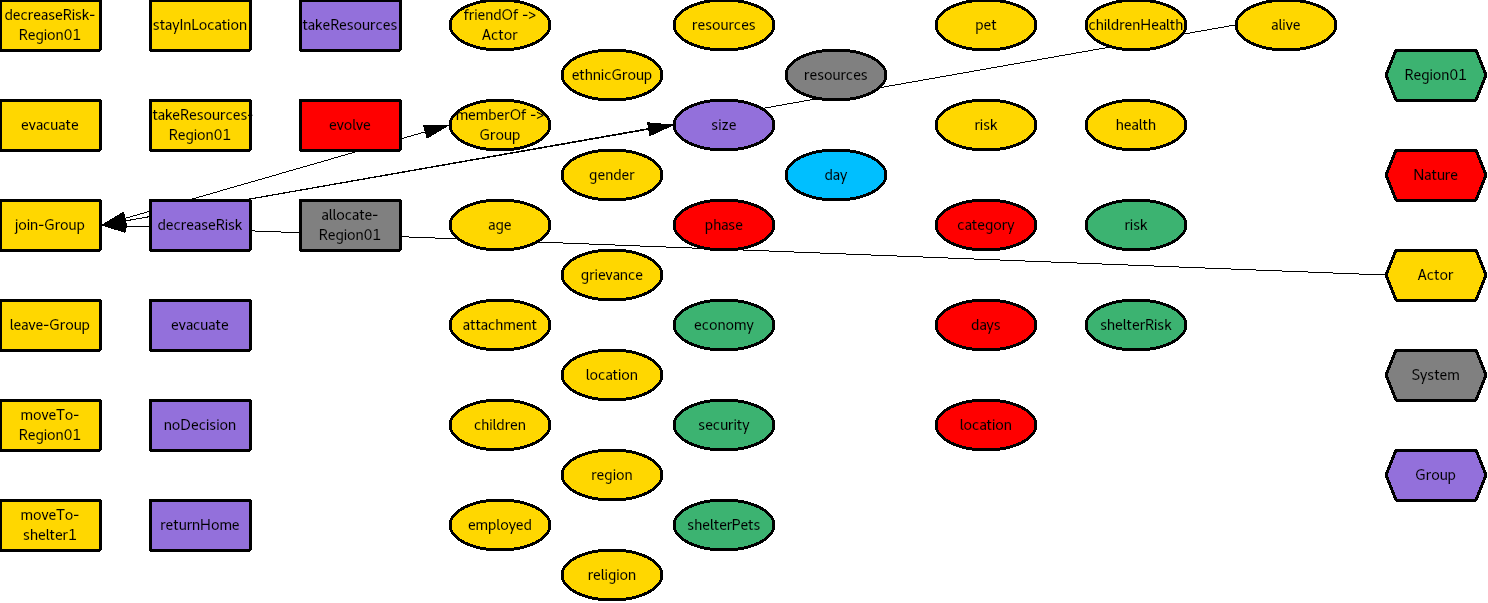
\includegraphics[width=0.8\textwidth]{images/Actor-join-Group.png}%
\caption{Ground Truth subgraph for Actor{-}join{-}Group}%
\end{figure}

%
\subsubsection{Applicability of Actor join Group}%
\label{ssubsec:Applicability of Actor join Group}%
\begin{flushleft}%
IF %
\textbf{Actor's alive}%
\linebreak%
\hspace*{2em}%
THEN %
IF %
\textbf{Actor memberOf Group}%
\linebreak%
\hspace*{4em}%
THEN %
\textbf{false}%
\linebreak%
\hspace*{4em}%
ELSE %
\textbf{true}%
\linebreak%
\hspace*{2em}%
ELSE %
\textbf{false}%
\end{flushleft}

%
\subsubsection{Effect on Actor memberOf Group of Actor join Group}%
\label{ssubsec:Effect on Actor memberOf Group of Actor join Group}%
\begin{flushleft}%
$\mbox{\textbf{Actor memberOf Group}} '$%
$\leftarrow$%
\textbf{true}%
\end{flushleft}

%
\subsubsection{Effect on Group's size of Actor join Group}%
\label{ssubsec:Effect on Group's size of Actor join Group}%
\begin{flushleft}%
$\mbox{\textbf{Group's size}} '$%
$\leftarrow$%
\textbf{Group's size}%
+1%
\end{flushleft}

%
\subsection{Actor leave Group}%
\label{subsec:Actor leave Group}%


\begin{figure}[ht]%
\centering%
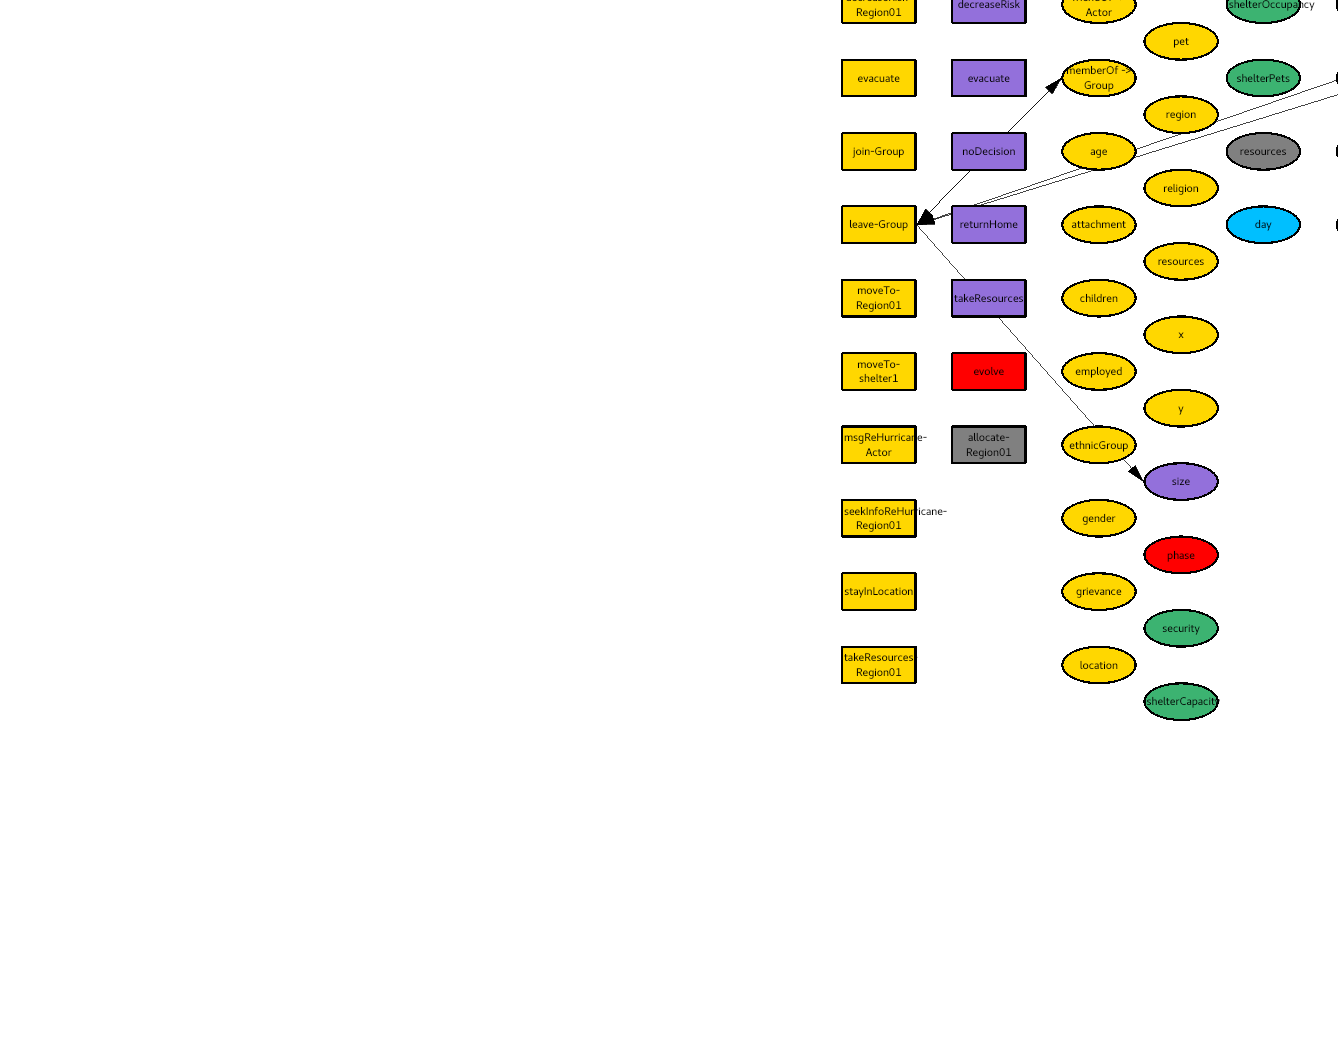
\includegraphics[width=0.8\textwidth]{images/Actor-leave-Group.png}%
\caption{Ground Truth subgraph for Actor{-}leave{-}Group}%
\end{figure}

%
\subsubsection{Applicability of Actor leave Group}%
\label{ssubsec:Applicability of Actor leave Group}%
\begin{flushleft}%
IF %
\textbf{Actor's alive}%
\linebreak%
\hspace*{2em}%
THEN %
IF %
\textbf{Actor memberOf Group}%
\linebreak%
\hspace*{4em}%
THEN %
\textbf{true}%
\linebreak%
\hspace*{4em}%
ELSE %
\textbf{false}%
\linebreak%
\hspace*{2em}%
ELSE %
\textbf{false}%
\end{flushleft}

%
\subsubsection{Effect on Actor memberOf Group of Actor leave Group}%
\label{ssubsec:Effect on Actor memberOf Group of Actor leave Group}%
\begin{flushleft}%
$\mbox{\textbf{Actor memberOf Group}} '$%
$\leftarrow$%
\textbf{false}%
\end{flushleft}

%
\subsubsection{Effect on Group's size of Actor leave Group}%
\label{ssubsec:Effect on Group's size of Actor leave Group}%
\begin{flushleft}%
$\mbox{\textbf{Group's size}} '$%
$\leftarrow$%
\textbf{Group's size}%
${-}1$%
\end{flushleft}

%
\subsection{Actor moveTo Region01}%
\label{subsec:Actor moveTo Region01}%


\begin{figure}[ht]%
\centering%
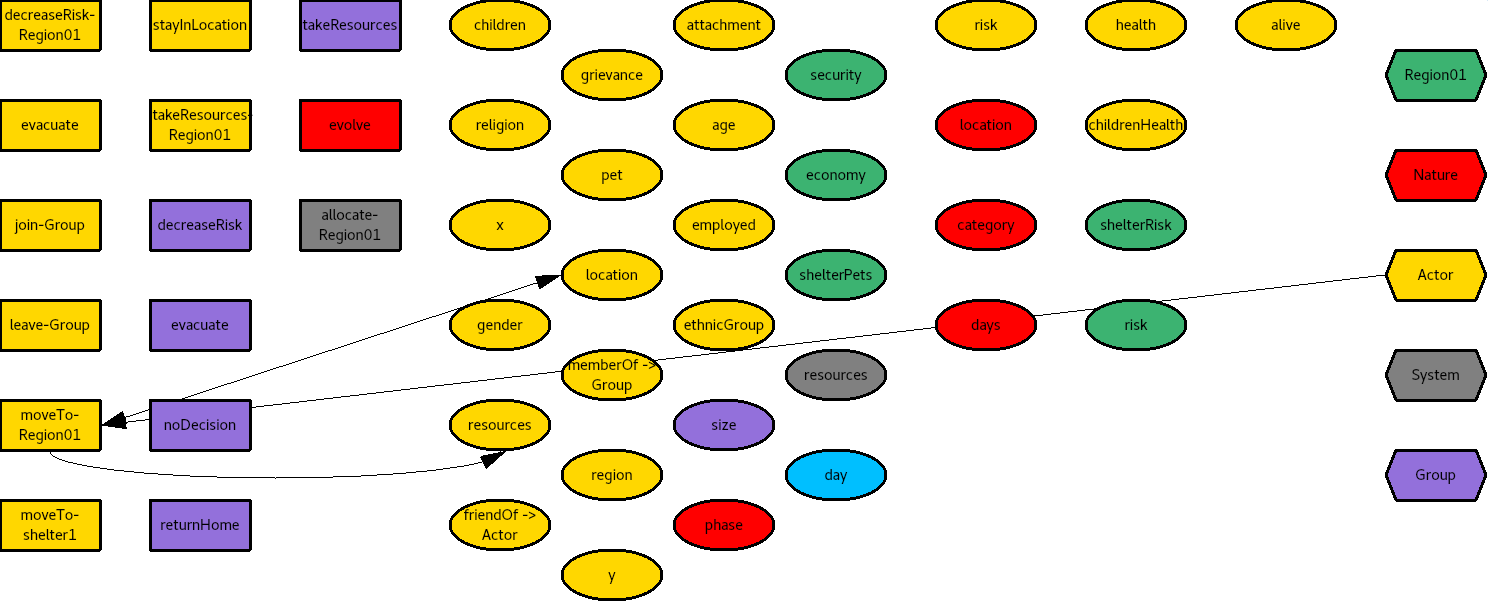
\includegraphics[width=0.8\textwidth]{images/Actor-moveTo-Region01.png}%
\caption{Ground Truth subgraph for Actor{-}moveTo{-}Region01}%
\end{figure}

%
\subsubsection{Applicability of Actor moveTo Region01}%
\label{ssubsec:Applicability of Actor moveTo Region01}%
\begin{flushleft}%
IF %
\textbf{Actor's location}%
$=$%
\textbf{\{'evacuated', 'shelter1'\}}%
\linebreak%
\hspace*{2em}%
THEN %
\textbf{true}%
\linebreak%
\hspace*{2em}%
ELSE %
\textbf{false}%
\end{flushleft}

%
\subsubsection{Effect on Actor's location of Actor moveTo Region01}%
\label{ssubsec:Effect on Actor's location of Actor moveTo Region01}%
\begin{flushleft}%
$\mbox{\textbf{Actor's location}} '$%
$\leftarrow$%
\textbf{Region01}%
\end{flushleft}

%
\subsubsection{Effect on Actor's resources of Actor moveTo Region01}%
\label{ssubsec:Effect on Actor's resources of Actor moveTo Region01}%
\begin{flushleft}%
IF %
\textbf{Actor's alive}%
\linebreak%
\hspace*{2em}%
THEN %
IF %
\textbf{Actor's employed}%
\linebreak%
\hspace*{4em}%
THEN %
$\mbox{\textbf{Actor's resources}} '$%
$\leftarrow$%
80\%%
$\cdot$%
\textbf{Actor's resources}%
+0.20%
\linebreak%
\hspace*{4em}%
ELSE %
$\mbox{\textbf{Actor's resources}} '$%
$\leftarrow$%
\textbf{Actor's resources}%
\linebreak%
\hspace*{2em}%
ELSE %
$\mbox{\textbf{Actor's resources}} '$%
$\leftarrow$%
\textbf{Actor's resources}%
\end{flushleft}

%
\subsection{Actor moveTo shelter1}%
\label{subsec:Actor moveTo shelter1}%


\begin{figure}[ht]%
\centering%
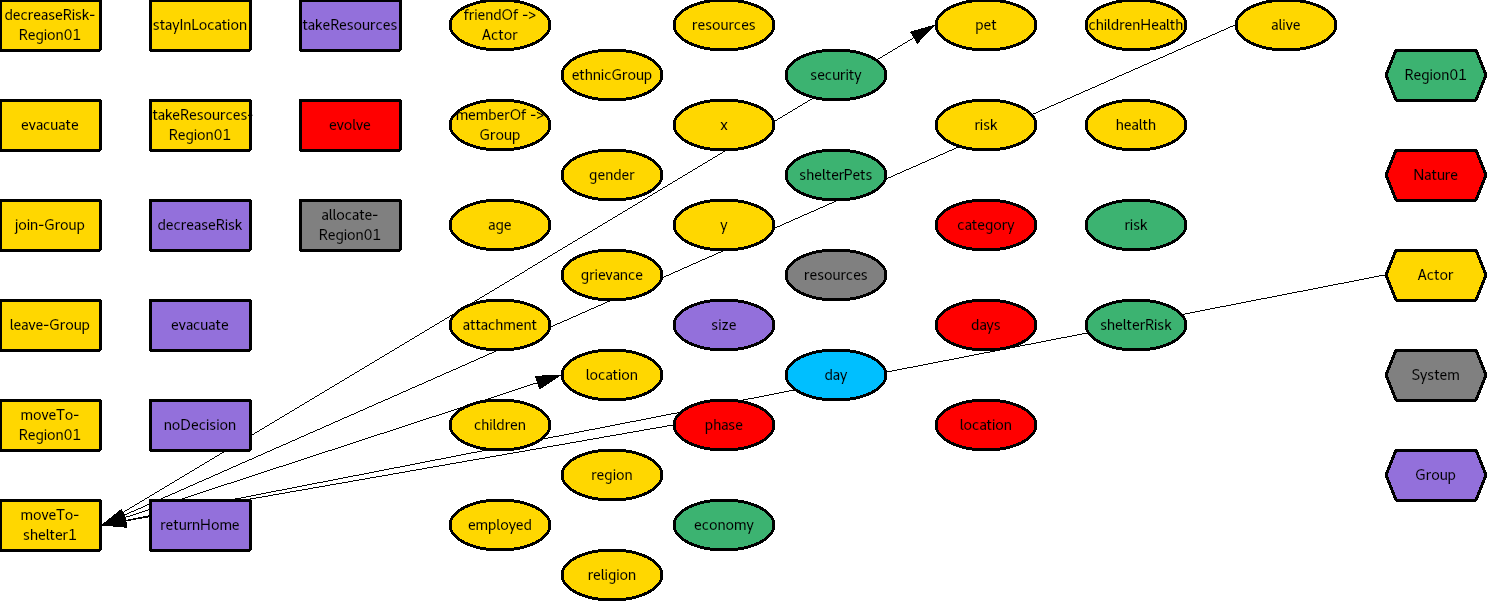
\includegraphics[width=0.8\textwidth]{images/Actor-moveTo-shelter1.png}%
\caption{Ground Truth subgraph for Actor{-}moveTo{-}shelter1}%
\end{figure}

%
\subsubsection{Applicability of Actor moveTo shelter1}%
\label{ssubsec:Applicability of Actor moveTo shelter1}%
\begin{flushleft}%
IF %
\textbf{Nature's phase}%
$=$%
\textbf{none}%
\linebreak%
\hspace*{2em}%
THEN %
\textbf{false}%
\linebreak%
\hspace*{2em}%
ELSE %
IF %
\textbf{Actor's alive}%
\linebreak%
\hspace*{4em}%
THEN %
IF %
\textbf{Actor's location}%
$=$%
\textbf{shelter1}%
\linebreak%
\hspace*{6em}%
THEN %
\textbf{false}%
\linebreak%
\hspace*{6em}%
ELSE %
\textbf{true}%
\linebreak%
\hspace*{4em}%
ELSE %
\textbf{false}%
\end{flushleft}

%
\subsubsection{Effect on Actor's location of Actor moveTo shelter1}%
\label{ssubsec:Effect on Actor's location of Actor moveTo shelter1}%
\begin{flushleft}%
$\mbox{\textbf{Actor's location}} '$%
$\leftarrow$%
\textbf{shelter1}%
\end{flushleft}

%
\subsection{Actor stayInLocation}%
\label{subsec:Actor stayInLocation}%


\begin{figure}[ht]%
\centering%
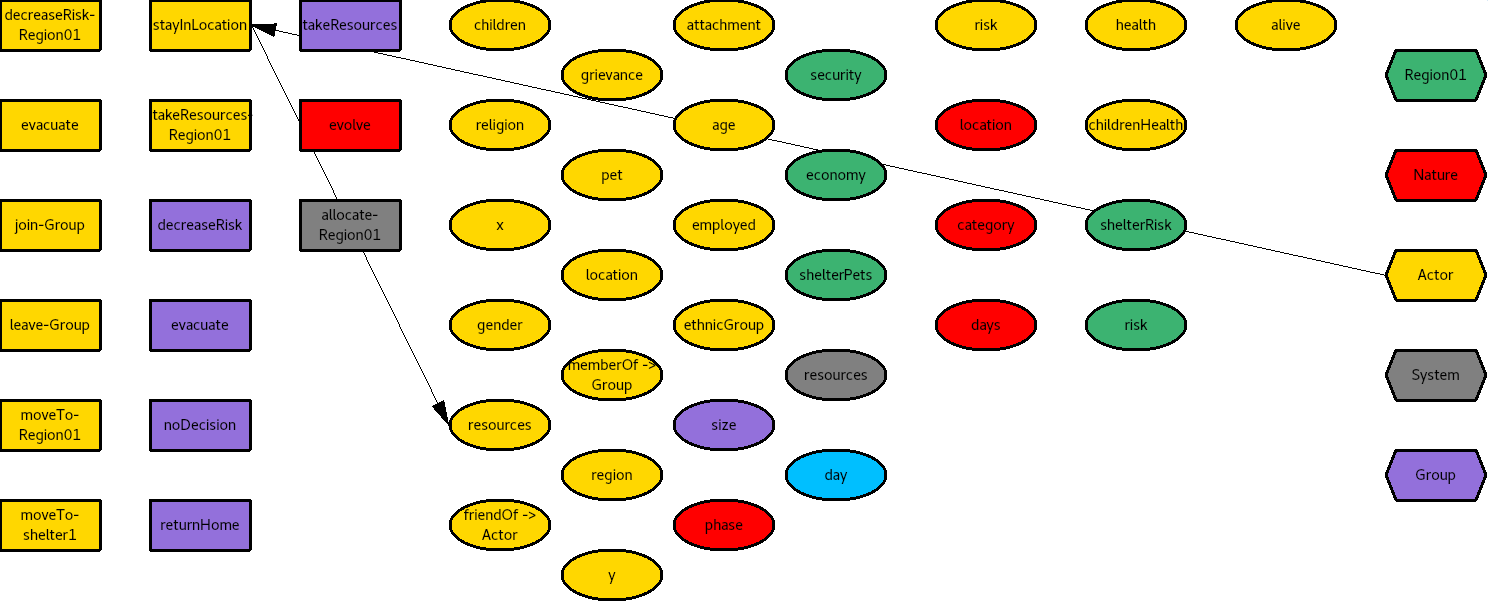
\includegraphics[width=0.8\textwidth]{images/Actor-stayInLocation.png}%
\caption{Ground Truth subgraph for Actor{-}stayInLocation}%
\end{figure}

%
\subsubsection{Effect on Actor's resources of Actor stayInLocation}%
\label{ssubsec:Effect on Actor's resources of Actor stayInLocation}%
\begin{flushleft}%
IF %
\textbf{Actor's alive}%
\linebreak%
\hspace*{2em}%
THEN %
IF %
\textbf{Actor's employed}%
\linebreak%
\hspace*{4em}%
THEN %
IF %
\textbf{Actor's location}%
$=$%
\textbf{\{'Region01', 'evacuated'\}}%
\linebreak%
\hspace*{6em}%
THEN %
$\mbox{\textbf{Actor's resources}} '$%
$\leftarrow$%
80\%%
$\cdot$%
\textbf{Actor's resources}%
+0.20%
\linebreak%
\hspace*{6em}%
ELSE %
$\mbox{\textbf{Actor's resources}} '$%
$\leftarrow$%
\textbf{Actor's resources}%
\linebreak%
\hspace*{4em}%
ELSE %
$\mbox{\textbf{Actor's resources}} '$%
$\leftarrow$%
\textbf{Actor's resources}%
\linebreak%
\hspace*{2em}%
ELSE %
$\mbox{\textbf{Actor's resources}} '$%
$\leftarrow$%
\textbf{Actor's resources}%
\end{flushleft}

%
\subsection{Actor takeResources Region01}%
\label{subsec:Actor takeResources Region01}%


\begin{figure}[ht]%
\centering%
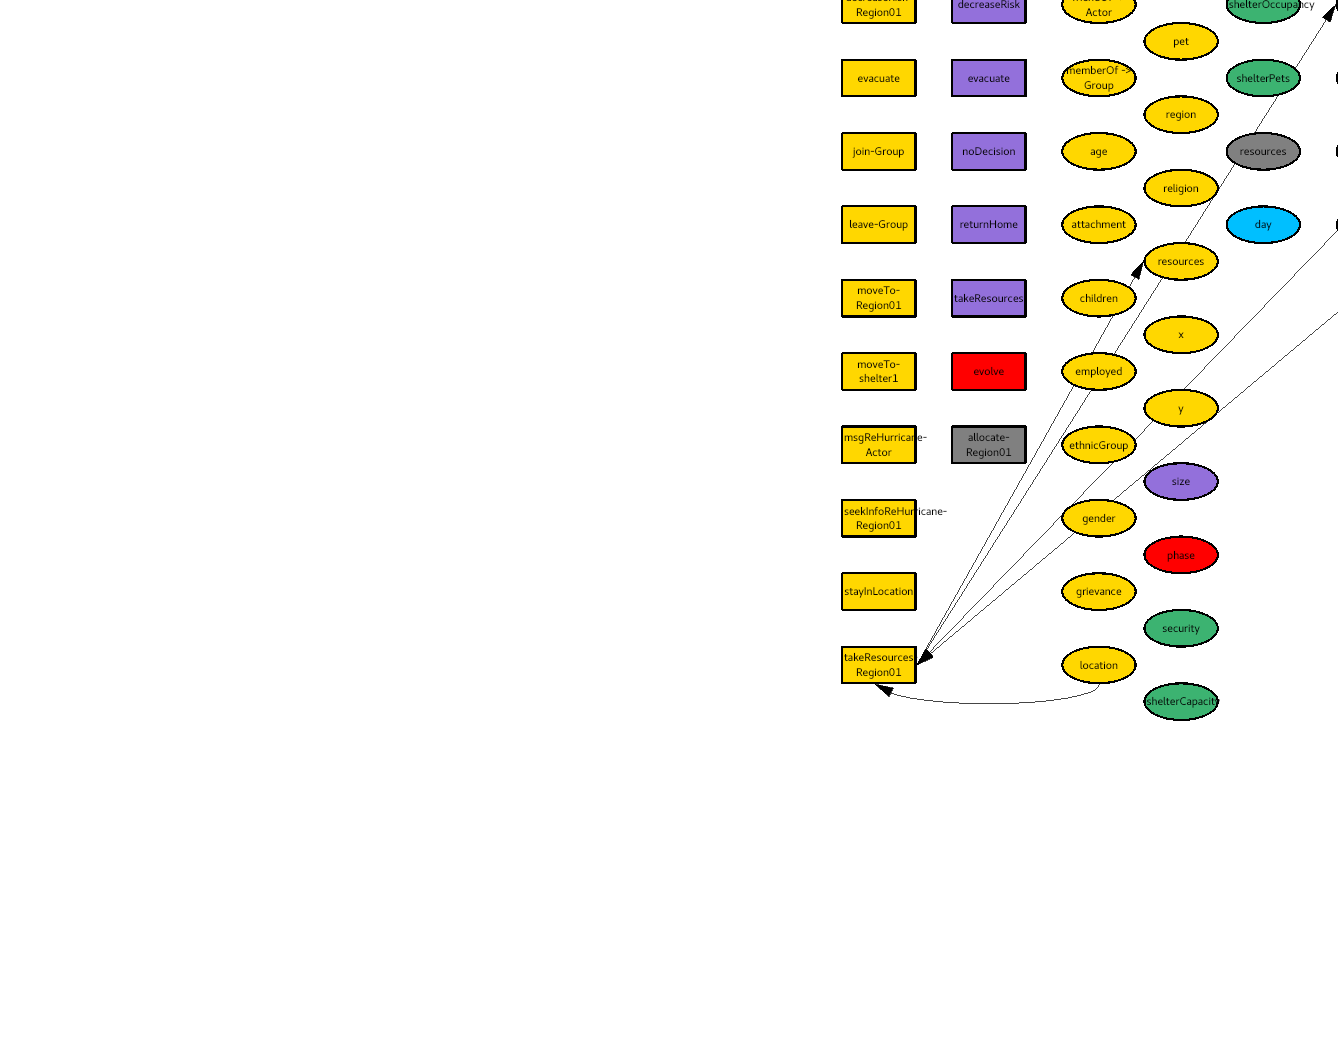
\includegraphics[width=0.8\textwidth]{images/Actor-takeResources-Region01.png}%
\caption{Ground Truth subgraph for Actor{-}takeResources{-}Region01}%
\end{figure}

%
\subsubsection{Applicability of Actor takeResources Region01}%
\label{ssubsec:Applicability of Actor takeResources Region01}%
\begin{flushleft}%
IF %
\textbf{Actor's location}%
$=$%
\textbf{Region01}%
\linebreak%
\hspace*{2em}%
THEN %
IF %
\textbf{Actor's alive}%
\linebreak%
\hspace*{4em}%
THEN %
\textbf{true}%
\linebreak%
\hspace*{4em}%
ELSE %
\textbf{false}%
\linebreak%
\hspace*{2em}%
ELSE %
\textbf{false}%
\end{flushleft}

%
\subsubsection{Effect on Actor's resources of Actor takeResources Region01}%
\label{ssubsec:Effect on Actor's resources of Actor takeResources Region01}%
\begin{flushleft}%
$\mbox{\textbf{Actor's resources}} '$%
$\leftarrow$%
80\%%
$\cdot$%
\textbf{Actor's resources}%
+0.20%
\end{flushleft}

%
\subsubsection{Effect on Actor's risk of Actor takeResources Region01}%
\label{ssubsec:Effect on Actor's risk of Actor takeResources Region01}%
\begin{flushleft}%
IF %
\textbf{Nature's phase}%
$=$%
\textbf{none}%
\linebreak%
\hspace*{2em}%
THEN %
$\mbox{\textbf{Actor's risk}} '$%
$\leftarrow$%
19\%%
$\cdot$%
\textbf{Actor's risk}%
+0.80%
\linebreak%
\hspace*{2em}%
ELSE %
$\mbox{\textbf{Actor's risk}} '$%
$\leftarrow$%
40\%%
$\cdot$%
\textbf{Actor's risk}%
+0.60%
\end{flushleft}

%
\subsection{System allocate Region01}%
\label{subsec:System allocate Region01}%


\begin{figure}[ht]%
\centering%
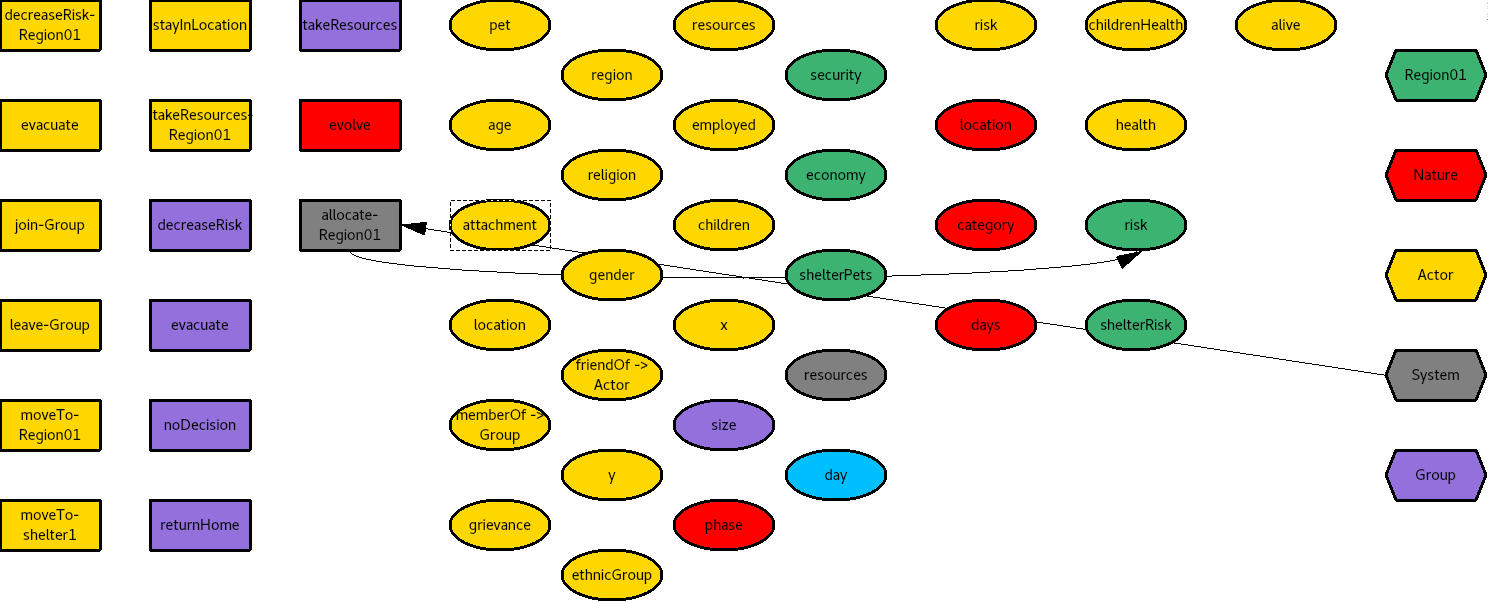
\includegraphics[width=0.8\textwidth]{images/System-allocate-Region01.png}%
\caption{Ground Truth subgraph for System{-}allocate{-}Region01}%
\end{figure}

%
\subsubsection{Effect on Region01's risk of System allocate Region01}%
\label{ssubsec:Effect on Region01's risk of System allocate Region01}%
\begin{flushleft}%
$\mbox{\textbf{Region01's risk}} '$%
$\leftarrow$%
80\%%
$\cdot$%
\textbf{Region01's risk}%
\end{flushleft}

%
\subsection{Group decreaseRisk}%
\label{subsec:Group decreaseRisk}%


\begin{figure}[ht]%
\centering%
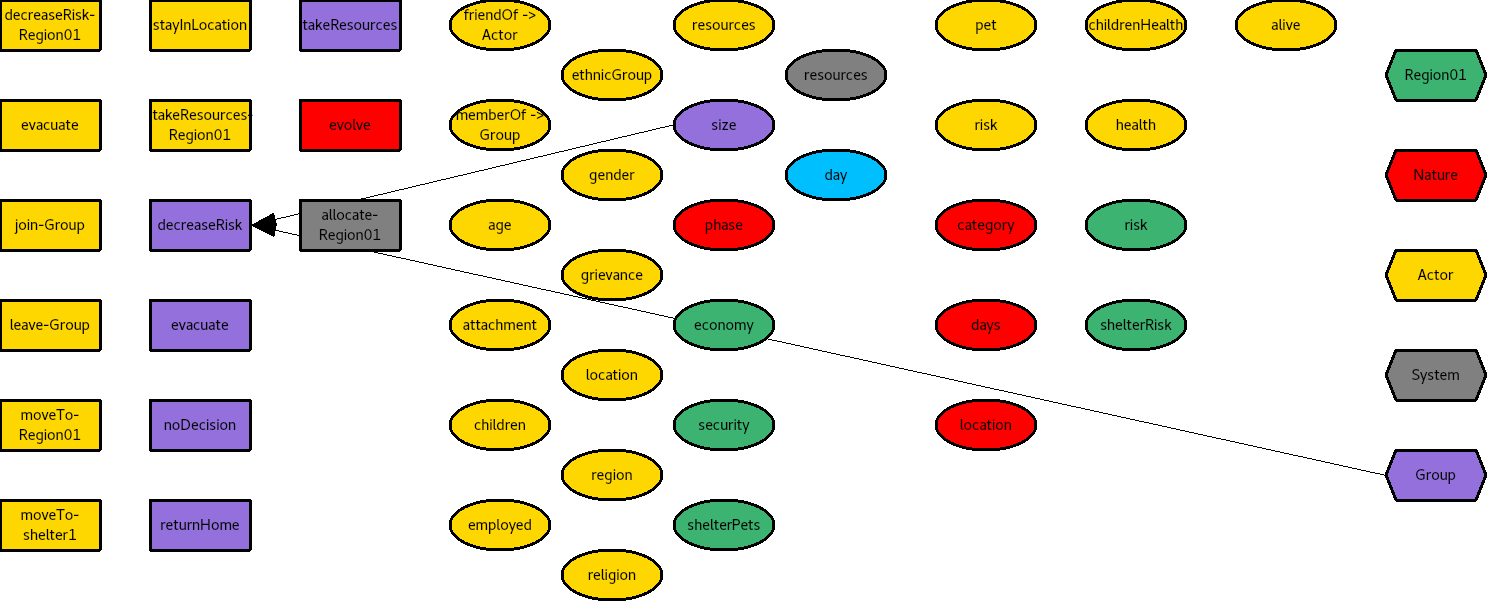
\includegraphics[width=0.8\textwidth]{images/Group-decreaseRisk.png}%
\caption{Ground Truth subgraph for Group{-}decreaseRisk}%
\end{figure}

%
\subsubsection{Applicability of Group decreaseRisk}%
\label{ssubsec:Applicability of Group decreaseRisk}%
\begin{flushleft}%
IF %
\textbf{Group's size}%
$>$%
0%
\linebreak%
\hspace*{2em}%
THEN %
\textbf{true}%
\linebreak%
\hspace*{2em}%
ELSE %
\textbf{false}%
\end{flushleft}

%
\subsection{Group evacuate}%
\label{subsec:Group evacuate}%


\begin{figure}[ht]%
\centering%
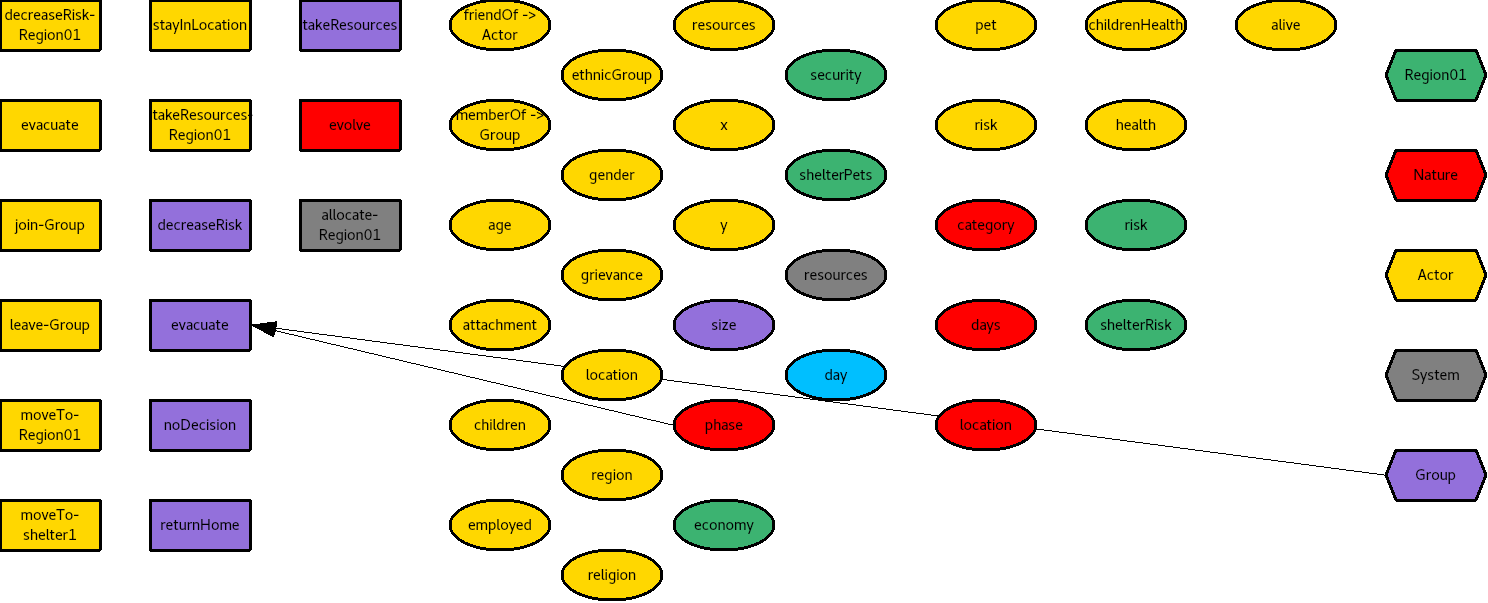
\includegraphics[width=0.8\textwidth]{images/Group-evacuate.png}%
\caption{Ground Truth subgraph for Group{-}evacuate}%
\end{figure}

%
\subsubsection{Applicability of Group evacuate}%
\label{ssubsec:Applicability of Group evacuate}%
\begin{flushleft}%
IF %
\textbf{Nature's phase}%
$=$%
\textbf{none}%
\linebreak%
\hspace*{2em}%
THEN %
\textbf{false}%
\linebreak%
\hspace*{2em}%
ELSE %
\textbf{true}%
\end{flushleft}

%
\subsection{Group noDecision}%
\label{subsec:Group noDecision}%


\begin{figure}[ht]%
\centering%
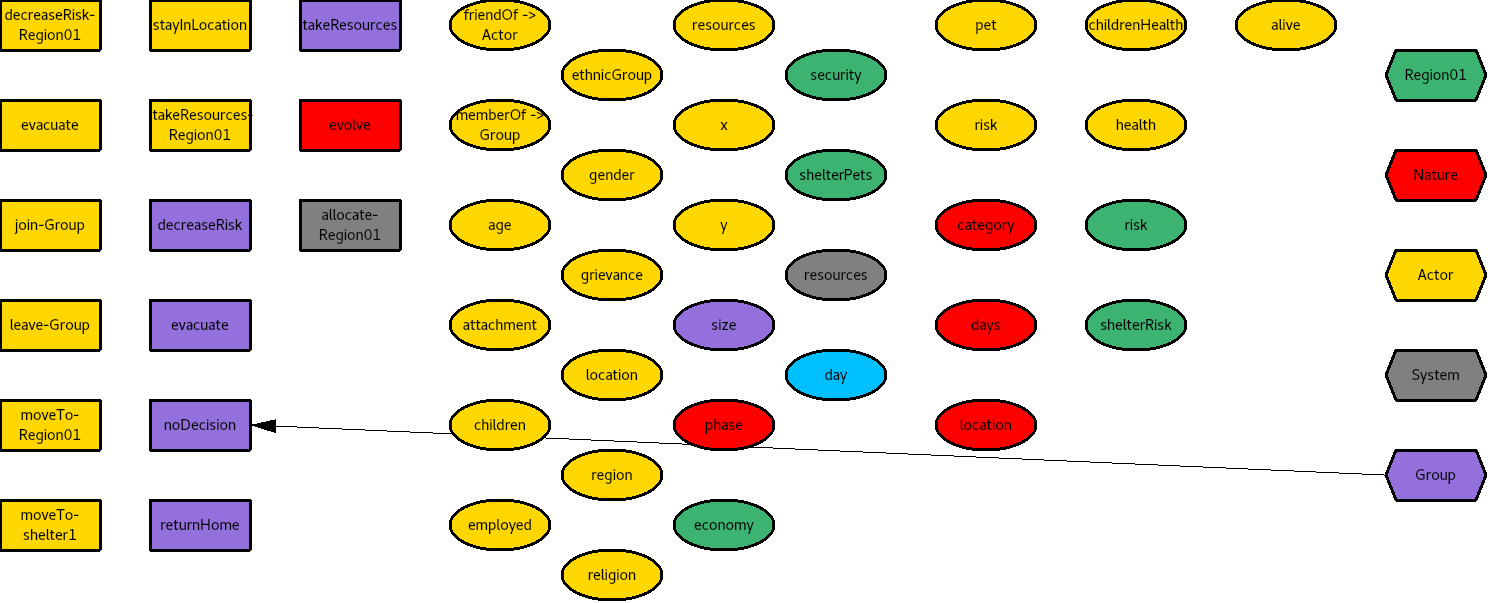
\includegraphics[width=0.8\textwidth]{images/Group-noDecision.png}%
\caption{Ground Truth subgraph for Group{-}noDecision}%
\end{figure}

%
\subsection{Group returnHome}%
\label{subsec:Group returnHome}%


\begin{figure}[ht]%
\centering%
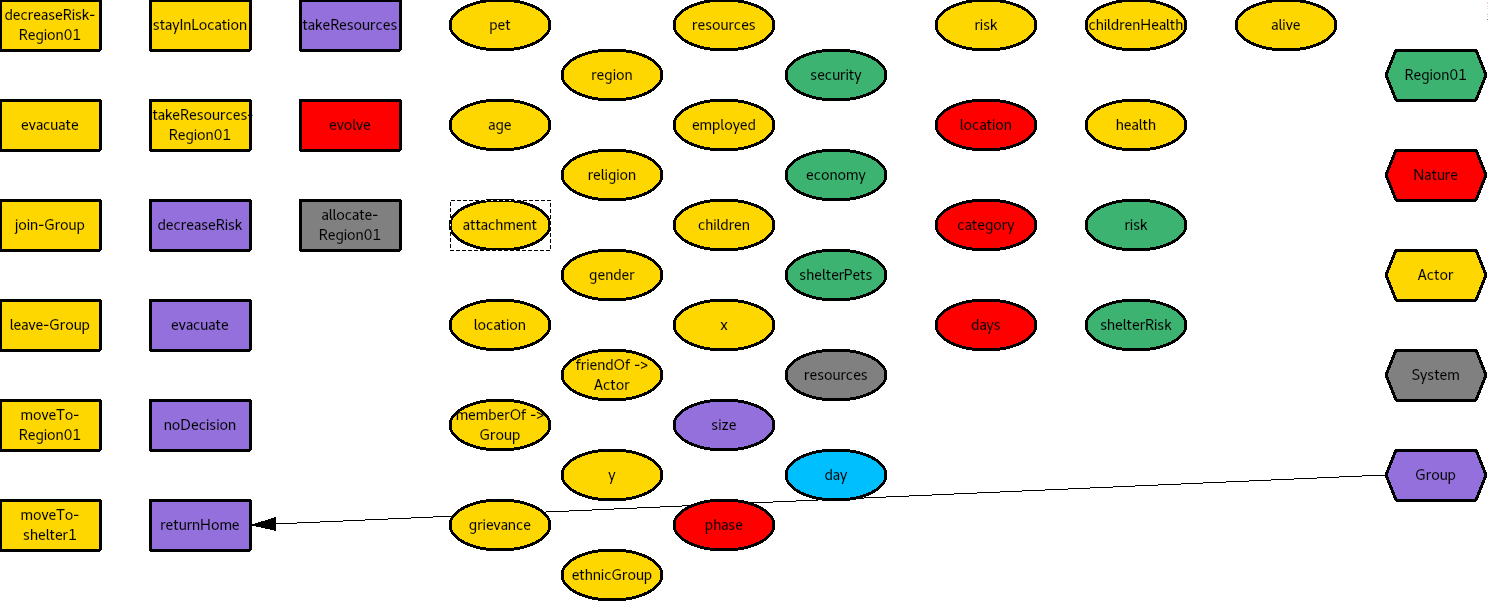
\includegraphics[width=0.8\textwidth]{images/Group-returnHome.png}%
\caption{Ground Truth subgraph for Group{-}returnHome}%
\end{figure}

%
\subsection{Group takeResources}%
\label{subsec:Group takeResources}%


\begin{figure}[ht]%
\centering%
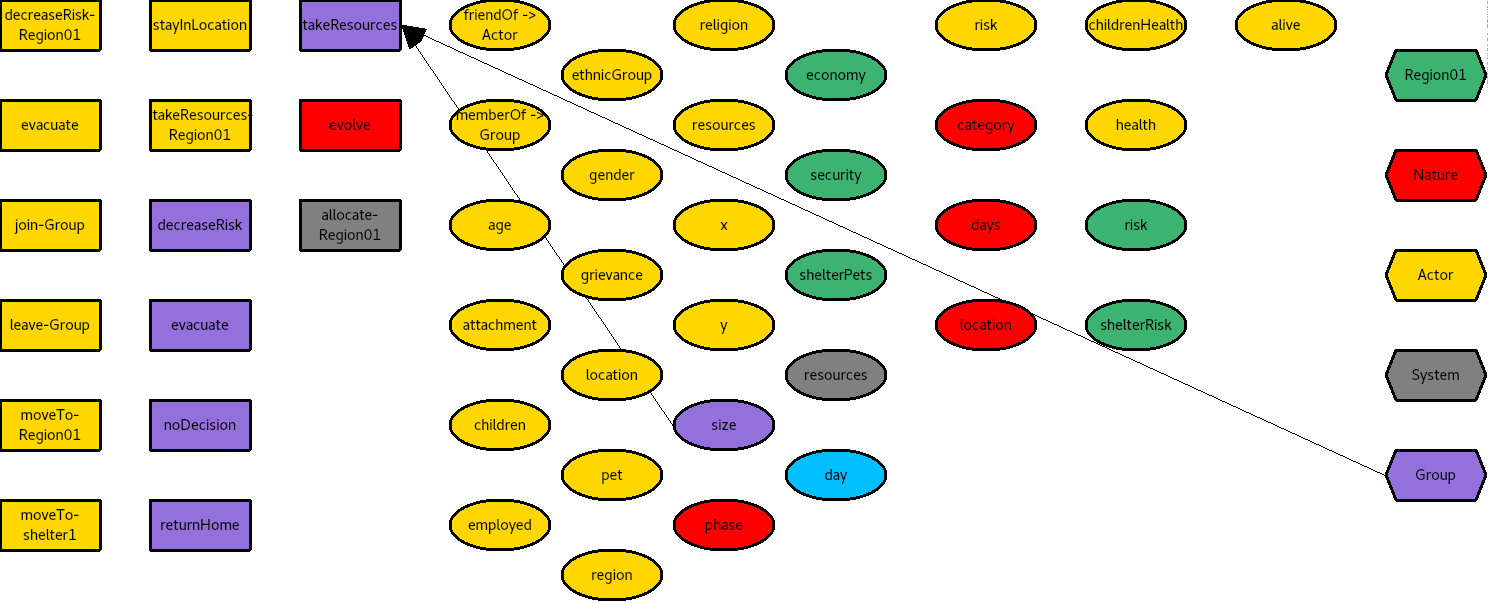
\includegraphics[width=0.8\textwidth]{images/Group-takeResources.png}%
\caption{Ground Truth subgraph for Group{-}takeResources}%
\end{figure}

%
\subsubsection{Applicability of Group takeResources}%
\label{ssubsec:Applicability of Group takeResources}%
\begin{flushleft}%
IF %
\textbf{Group's size}%
$>$%
0%
\linebreak%
\hspace*{2em}%
THEN %
\textbf{true}%
\linebreak%
\hspace*{2em}%
ELSE %
\textbf{false}%
\end{flushleft}

%
\section{Expected Reward}%
\label{sec:Expected Reward}%
\subsection{Actor's Reward}%
\label{subsec:Actor's Reward}%


\begin{figure}[ht]%
\centering%
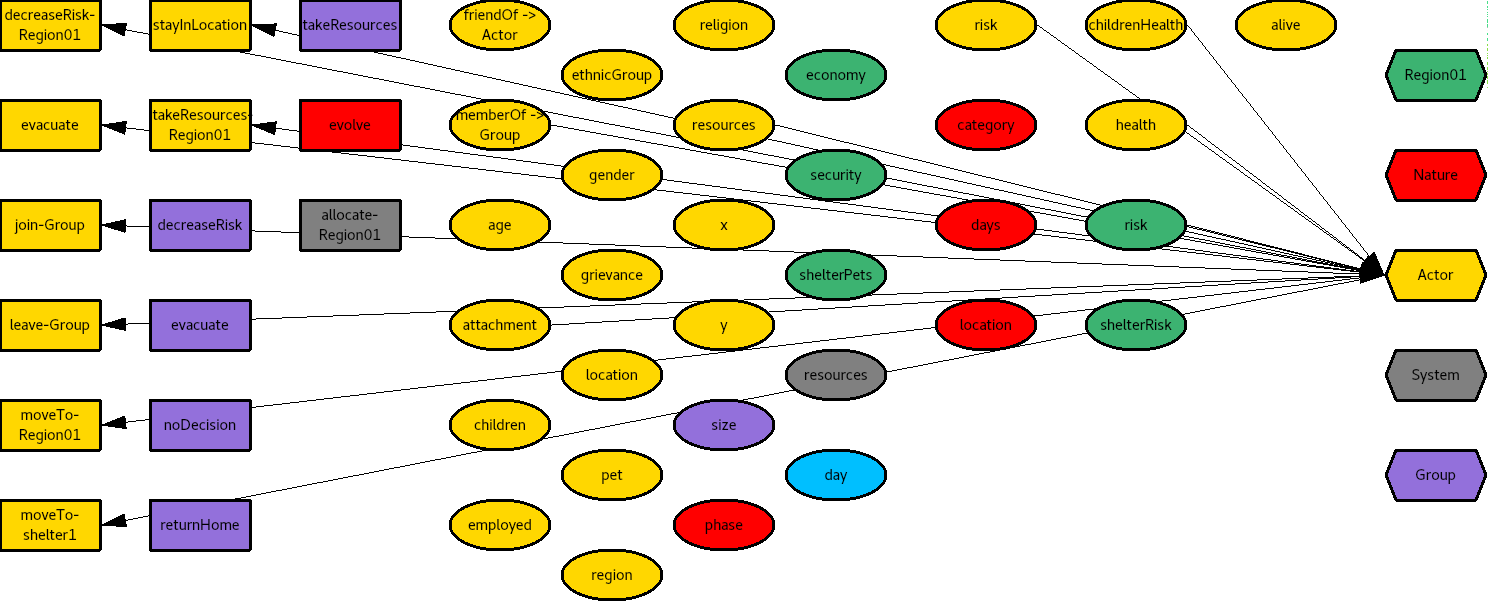
\includegraphics[width=0.8\textwidth]{images/Actor.png}%
\caption{Ground Truth subgraph for Actor}%
\end{figure}

%
\begin{flushleft}%
IF %
\textbf{Actor's risk}%
$>$%
0.60%
\linebreak%
\hspace*{2em}%
THEN %
IF %
\textbf{Actor's attachment}%
$=$%
\textbf{anxious}%
\linebreak%
\hspace*{4em}%
THEN %
$R$%
$\leftarrow$%
20\%%
$\cdot$%
\textbf{Actor memberOf Group}%
+%
40\%%
$\cdot$%
\textbf{Actor's childrenHealth}%
+%
60\%%
$\cdot$%
\textbf{Actor's health}%
+%
20\%%
$\cdot$%
\textbf{Actor's resources}%
+%
{-}60\%%
$\cdot$%
\textbf{Region01's risk}%
\linebreak%
\hspace*{4em}%
ELSE %
IF %
\textbf{Actor's attachment}%
$=$%
\textbf{avoidant}%
\linebreak%
\hspace*{6em}%
THEN %
$R$%
$\leftarrow$%
{-}20\%%
$\cdot$%
\textbf{Actor memberOf Group}%
+%
40\%%
$\cdot$%
\textbf{Actor's childrenHealth}%
+%
60\%%
$\cdot$%
\textbf{Actor's health}%
+%
20\%%
$\cdot$%
\textbf{Actor's resources}%
+%
{-}60\%%
$\cdot$%
\textbf{Region01's risk}%
\linebreak%
\hspace*{6em}%
ELSE %
$R$%
$\leftarrow$%
40\%%
$\cdot$%
\textbf{Actor's childrenHealth}%
+%
60\%%
$\cdot$%
\textbf{Actor's health}%
+%
20\%%
$\cdot$%
\textbf{Actor's resources}%
+%
{-}60\%%
$\cdot$%
\textbf{Region01's risk}%
\linebreak%
\hspace*{2em}%
ELSE %
$R$%
$\leftarrow$%
40\%%
$\cdot$%
\textbf{Actor's childrenHealth}%
+%
60\%%
$\cdot$%
\textbf{Actor's health}%
+%
20\%%
$\cdot$%
\textbf{Actor's resources}%
+%
{-}60\%%
$\cdot$%
\textbf{Region01's risk}%
\end{flushleft}

%
\subsection{Group's Reward}%
\label{subsec:Group's Reward}%


\begin{figure}[ht]%
\centering%
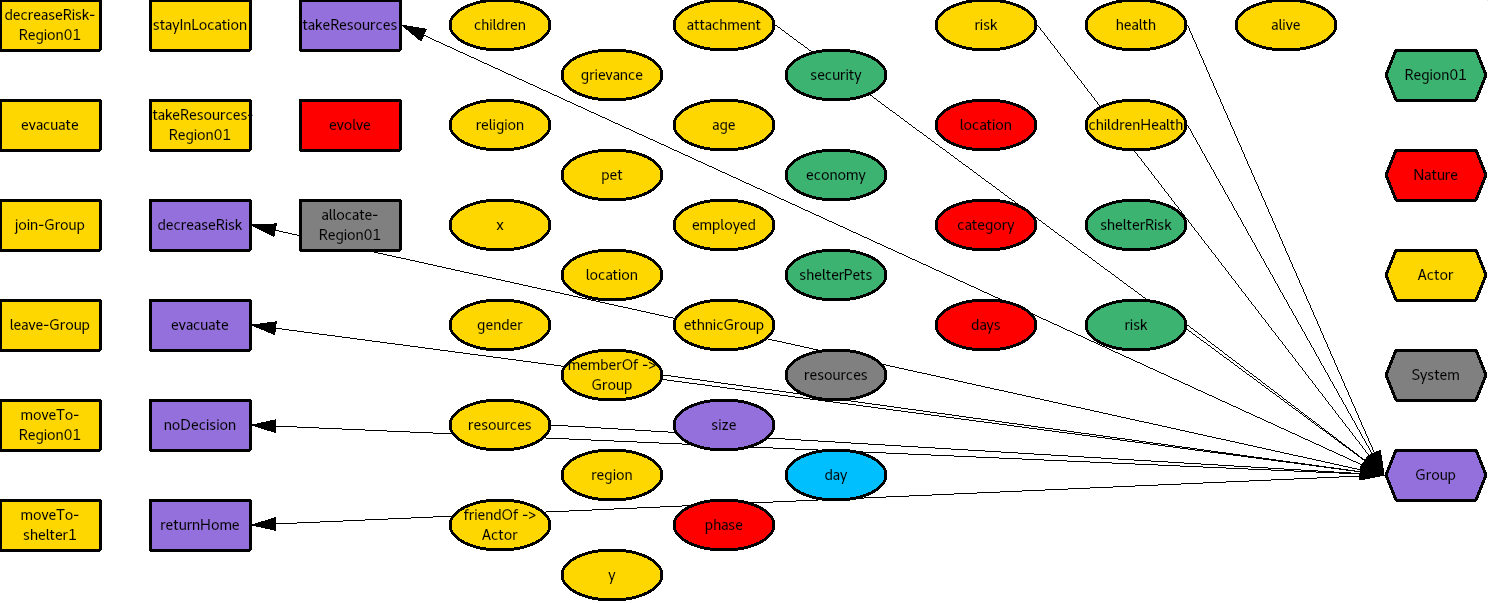
\includegraphics[width=0.8\textwidth]{images/Group.png}%
\caption{Ground Truth subgraph for Group}%
\end{figure}

%
\begin{flushleft}%
IF %
\textbf{Actor's risk}%
$>$%
0.60%
\linebreak%
\hspace*{2em}%
THEN %
IF %
\textbf{Actor's attachment}%
$=$%
\textbf{anxious}%
\linebreak%
\hspace*{4em}%
THEN %
$R$%
$\leftarrow$%
20\%%
$\cdot$%
\textbf{Actor memberOf Group}%
+%
40\%%
$\cdot$%
\textbf{Actor's childrenHealth}%
+%
60\%%
$\cdot$%
\textbf{Actor's health}%
+%
20\%%
$\cdot$%
\textbf{Actor's resources}%
+%
{-}60\%%
$\cdot$%
\textbf{Region01's risk}%
\linebreak%
\hspace*{4em}%
ELSE %
IF %
\textbf{Actor's attachment}%
$=$%
\textbf{avoidant}%
\linebreak%
\hspace*{6em}%
THEN %
$R$%
$\leftarrow$%
{-}20\%%
$\cdot$%
\textbf{Actor memberOf Group}%
+%
40\%%
$\cdot$%
\textbf{Actor's childrenHealth}%
+%
60\%%
$\cdot$%
\textbf{Actor's health}%
+%
20\%%
$\cdot$%
\textbf{Actor's resources}%
+%
{-}60\%%
$\cdot$%
\textbf{Region01's risk}%
\linebreak%
\hspace*{6em}%
ELSE %
$R$%
$\leftarrow$%
40\%%
$\cdot$%
\textbf{Actor's childrenHealth}%
+%
60\%%
$\cdot$%
\textbf{Actor's health}%
+%
20\%%
$\cdot$%
\textbf{Actor's resources}%
+%
{-}60\%%
$\cdot$%
\textbf{Region01's risk}%
\linebreak%
\hspace*{2em}%
ELSE %
$R$%
$\leftarrow$%
40\%%
$\cdot$%
\textbf{Actor's childrenHealth}%
+%
60\%%
$\cdot$%
\textbf{Actor's health}%
+%
20\%%
$\cdot$%
\textbf{Actor's resources}%
+%
{-}60\%%
$\cdot$%
\textbf{Region01's risk}%
\end{flushleft}

%
\end{document}